\documentclass[twoside]{book}

% Packages required by doxygen
\usepackage{fixltx2e}
\usepackage{calc}
\usepackage{doxygen}
\usepackage[export]{adjustbox} % also loads graphicx
\usepackage{graphicx}
\usepackage[utf8]{inputenc}
\usepackage{makeidx}
\usepackage{multicol}
\usepackage{multirow}
\PassOptionsToPackage{warn}{textcomp}
\usepackage{textcomp}
\usepackage[nointegrals]{wasysym}
\usepackage[table]{xcolor}

% Font selection
\usepackage[T1]{fontenc}
\usepackage[scaled=.90]{helvet}
\usepackage{courier}
\usepackage{amssymb}
\usepackage{sectsty}
\renewcommand{\familydefault}{\sfdefault}
\allsectionsfont{%
  \fontseries{bc}\selectfont%
  \color{darkgray}%
}
\renewcommand{\DoxyLabelFont}{%
  \fontseries{bc}\selectfont%
  \color{darkgray}%
}
\newcommand{\+}{\discretionary{\mbox{\scriptsize$\hookleftarrow$}}{}{}}

% Page & text layout
\usepackage{geometry}
\geometry{%
  a4paper,%
  top=2.5cm,%
  bottom=2.5cm,%
  left=2.5cm,%
  right=2.5cm%
}
\tolerance=750
\hfuzz=15pt
\hbadness=750
\setlength{\emergencystretch}{15pt}
\setlength{\parindent}{0cm}
\setlength{\parskip}{0.2cm}
\makeatletter
\renewcommand{\paragraph}{%
  \@startsection{paragraph}{4}{0ex}{-1.0ex}{1.0ex}{%
    \normalfont\normalsize\bfseries\SS@parafont%
  }%
}
\renewcommand{\subparagraph}{%
  \@startsection{subparagraph}{5}{0ex}{-1.0ex}{1.0ex}{%
    \normalfont\normalsize\bfseries\SS@subparafont%
  }%
}
\makeatother

% Headers & footers
\usepackage{fancyhdr}
\pagestyle{fancyplain}
\fancyhead[LE]{\fancyplain{}{\bfseries\thepage}}
\fancyhead[CE]{\fancyplain{}{}}
\fancyhead[RE]{\fancyplain{}{\bfseries\leftmark}}
\fancyhead[LO]{\fancyplain{}{\bfseries\rightmark}}
\fancyhead[CO]{\fancyplain{}{}}
\fancyhead[RO]{\fancyplain{}{\bfseries\thepage}}
\fancyfoot[LE]{\fancyplain{}{}}
\fancyfoot[CE]{\fancyplain{}{}}
\fancyfoot[RE]{\fancyplain{}{\bfseries\scriptsize Generated on Sat Jun 20 2015 19\+:35\+:50 for Eye\+Kin by Doxygen }}
\fancyfoot[LO]{\fancyplain{}{\bfseries\scriptsize Generated on Sat Jun 20 2015 19\+:35\+:50 for Eye\+Kin by Doxygen }}
\fancyfoot[CO]{\fancyplain{}{}}
\fancyfoot[RO]{\fancyplain{}{}}
\renewcommand{\footrulewidth}{0.4pt}
\renewcommand{\chaptermark}[1]{%
  \markboth{#1}{}%
}
\renewcommand{\sectionmark}[1]{%
  \markright{\thesection\ #1}%
}

% Indices & bibliography
\usepackage{natbib}
\usepackage[titles]{tocloft}
\setcounter{tocdepth}{3}
\setcounter{secnumdepth}{5}
\makeindex

% Hyperlinks (required, but should be loaded last)
\usepackage{ifpdf}
\ifpdf
  \usepackage[pdftex,pagebackref=true]{hyperref}
\else
  \usepackage[ps2pdf,pagebackref=true]{hyperref}
\fi
\hypersetup{%
  colorlinks=true,%
  linkcolor=blue,%
  citecolor=blue,%
  unicode%
}

% Custom commands
\newcommand{\clearemptydoublepage}{%
  \newpage{\pagestyle{empty}\cleardoublepage}%
}


%===== C O N T E N T S =====

\begin{document}

% Titlepage & ToC
\hypersetup{pageanchor=false,
             bookmarks=true,
             bookmarksnumbered=true,
             pdfencoding=unicode
            }
\pagenumbering{roman}
\begin{titlepage}
\vspace*{7cm}
\begin{center}%
{\Large Eye\+Kin }\\
\vspace*{1cm}
{\large Generated by Doxygen 1.8.9.1}\\
\vspace*{0.5cm}
{\small Sat Jun 20 2015 19:35:50}\\
\end{center}
\end{titlepage}
\clearemptydoublepage
\tableofcontents
\clearemptydoublepage
\pagenumbering{arabic}
\hypersetup{pageanchor=true}

%--- Begin generated contents ---
\chapter{Namespace Index}
\section{Namespace List}
Here is a list of all documented namespaces with brief descriptions\+:\begin{DoxyCompactList}
\item\contentsline{section}{\hyperlink{namespacepersonal_robotics}{personal\+Robotics} \\*Defines a namespace to contain non project specific functionality developed at Personal Robotics Lab }{\pageref{dc/d3f/namespacepersonal_robotics}}{}
\end{DoxyCompactList}

\chapter{Hierarchical Index}
\section{Class Hierarchy}
This inheritance list is sorted roughly, but not completely, alphabetically\+:\begin{DoxyCompactList}
\item \contentsline{section}{personal\+Robotics\+:\+:Entity}{\pageref{classpersonal_robotics_1_1_entity}}{}
\item std\+:\+:exception\begin{DoxyCompactList}
\item \contentsline{section}{personal\+Robotics\+:\+:Socket\+Exception}{\pageref{classpersonal_robotics_1_1_socket_exception}}{}
\end{DoxyCompactList}
\item \contentsline{section}{personal\+Robotics\+:\+:Eye\+Kin}{\pageref{classpersonal_robotics_1_1_eye_kin}}{}
\item \contentsline{section}{personal\+Robotics\+:\+:I\+D\+Look\+Up}{\pageref{structpersonal_robotics_1_1_i_d_look_up}}{}
\item \contentsline{section}{personal\+Robotics\+:\+:Kinect\+Reader}{\pageref{classpersonal_robotics_1_1_kinect_reader}}{}
\begin{DoxyCompactList}
\item \contentsline{section}{personal\+Robotics\+:\+:Object\+Segmentor}{\pageref{classpersonal_robotics_1_1_object_segmentor}}{}
\end{DoxyCompactList}
\item \contentsline{section}{personal\+Robotics\+:\+:Mutex\+Type$<$ T $>$}{\pageref{classpersonal_robotics_1_1_mutex_type}}{}
\item \contentsline{section}{personal\+Robotics\+:\+:Mutex\+Type$<$ bool $>$}{\pageref{classpersonal_robotics_1_1_mutex_type}}{}
\item \contentsline{section}{personal\+Robotics\+:\+:Mutex\+Type$<$ int $>$}{\pageref{classpersonal_robotics_1_1_mutex_type}}{}
\item \contentsline{section}{personal\+Robotics\+:\+:Pose2\+Dim}{\pageref{structpersonal_robotics_1_1_pose2_dim}}{}
\item \contentsline{section}{personal\+Robotics\+:\+:Tcp}{\pageref{classpersonal_robotics_1_1_tcp}}{}
\begin{DoxyCompactList}
\item \contentsline{section}{personal\+Robotics\+:\+:Tcp\+Server}{\pageref{classpersonal_robotics_1_1_tcp_server}}{}
\end{DoxyCompactList}
\item \contentsline{section}{personal\+Robotics\+:\+:Timer}{\pageref{classpersonal_robotics_1_1_timer}}{}
\end{DoxyCompactList}

\chapter{Class Index}
\section{Class List}
Here are the classes, structs, unions and interfaces with brief descriptions\+:\begin{DoxyCompactList}
\item\contentsline{section}{\hyperlink{classpersonal_robotics_1_1_entity}{personal\+Robotics\+::\+Entity} }{\pageref{d2/dfa/classpersonal_robotics_1_1_entity}}{}
\item\contentsline{section}{\hyperlink{classpersonal_robotics_1_1_eye_kin}{personal\+Robotics\+::\+Eye\+Kin} }{\pageref{d7/ded/classpersonal_robotics_1_1_eye_kin}}{}
\item\contentsline{section}{\hyperlink{structpersonal_robotics_1_1_i_d_look_up}{personal\+Robotics\+::\+I\+D\+Look\+Up} \\*Stores characteristic information regarding an \hyperlink{classpersonal_robotics_1_1_entity}{Entity} }{\pageref{dd/db9/structpersonal_robotics_1_1_i_d_look_up}}{}
\item\contentsline{section}{\hyperlink{classpersonal_robotics_1_1_kinect_reader}{personal\+Robotics\+::\+Kinect\+Reader} \\*This class provides an polling based interface to retrieve image frames from Kinect v2.\+0 for Windows(8.\+1) }{\pageref{d2/d0e/classpersonal_robotics_1_1_kinect_reader}}{}
\item\contentsline{section}{\hyperlink{classpersonal_robotics_1_1_mutex_type}{personal\+Robotics\+::\+Mutex\+Type$<$ T $>$} }{\pageref{da/d1f/classpersonal_robotics_1_1_mutex_type}}{}
\item\contentsline{section}{\hyperlink{classpersonal_robotics_1_1_object_segmentor}{personal\+Robotics\+::\+Object\+Segmentor} }{\pageref{d5/d3a/classpersonal_robotics_1_1_object_segmentor}}{}
\item\contentsline{section}{\hyperlink{structpersonal_robotics_1_1_pose2_dim}{personal\+Robotics\+::\+Pose2\+Dim} }{\pageref{de/d28/structpersonal_robotics_1_1_pose2_dim}}{}
\item\contentsline{section}{\hyperlink{classpersonal_robotics_1_1_socket_exception}{personal\+Robotics\+::\+Socket\+Exception} }{\pageref{dd/d85/classpersonal_robotics_1_1_socket_exception}}{}
\item\contentsline{section}{\hyperlink{classpersonal_robotics_1_1_tcp}{personal\+Robotics\+::\+Tcp} }{\pageref{de/dd4/classpersonal_robotics_1_1_tcp}}{}
\item\contentsline{section}{\hyperlink{classpersonal_robotics_1_1_tcp_server}{personal\+Robotics\+::\+Tcp\+Server} }{\pageref{d2/d19/classpersonal_robotics_1_1_tcp_server}}{}
\item\contentsline{section}{\hyperlink{classpersonal_robotics_1_1_timer}{personal\+Robotics\+::\+Timer} }{\pageref{de/df6/classpersonal_robotics_1_1_timer}}{}
\end{DoxyCompactList}

\chapter{Namespace Documentation}
\hypertarget{namespacepersonal_robotics}{}\section{personal\+Robotics Namespace Reference}
\label{namespacepersonal_robotics}\index{personal\+Robotics@{personal\+Robotics}}


Defines a namespace to contain non project specific functionality developed at Personal Robotics Lab.  


\subsection*{Classes}
\begin{DoxyCompactItemize}
\item 
class \hyperlink{classpersonal_robotics_1_1_entity}{Entity}
\item 
class \hyperlink{classpersonal_robotics_1_1_eye_kin}{Eye\+Kin}
\item 
struct \hyperlink{structpersonal_robotics_1_1_i_d_look_up}{I\+D\+Look\+Up}
\begin{DoxyCompactList}\small\item\em Stores characteristic information regarding an \hyperlink{classpersonal_robotics_1_1_entity}{Entity}. \end{DoxyCompactList}\item 
class \hyperlink{classpersonal_robotics_1_1_kinect_reader}{Kinect\+Reader}
\begin{DoxyCompactList}\small\item\em This class provides an polling based interface to retrieve image frames from Kinect v2.\+0 for Windows(8.\+1) \end{DoxyCompactList}\item 
class \hyperlink{classpersonal_robotics_1_1_mutex_type}{Mutex\+Type}
\item 
class \hyperlink{classpersonal_robotics_1_1_object_segmentor}{Object\+Segmentor}
\item 
struct \hyperlink{structpersonal_robotics_1_1_pose2_dim}{Pose2\+Dim}
\item 
class \hyperlink{classpersonal_robotics_1_1_socket_exception}{Socket\+Exception}
\item 
class \hyperlink{classpersonal_robotics_1_1_tcp}{Tcp}
\item 
class \hyperlink{classpersonal_robotics_1_1_tcp_server}{Tcp\+Server}
\item 
class \hyperlink{classpersonal_robotics_1_1_timer}{Timer}
\end{DoxyCompactItemize}
\subsection*{Typedefs}
\begin{DoxyCompactItemize}
\item 
\hypertarget{namespacepersonal_robotics_a1ef569ada10ae2d7dbbb214211e23e37}{}typedef \hyperlink{classpersonal_robotics_1_1_mutex_type}{Mutex\+Type}$<$ bool $>$ {\bfseries Mutex\+Bool}\label{namespacepersonal_robotics_a1ef569ada10ae2d7dbbb214211e23e37}

\end{DoxyCompactItemize}
\subsection*{Functions}
\begin{DoxyCompactItemize}
\item 
{\footnotesize template$<$class Interface $>$ }\\void \hyperlink{namespacepersonal_robotics_a10bc590dad378d8a84fd97546b331d62}{safe\+Release} (Interface in\+Interface)
\begin{DoxyCompactList}\small\item\em Safely releases dynamically allocated interfaces. \end{DoxyCompactList}\item 
\hypertarget{namespacepersonal_robotics_a2c3daa4285088463c734b34b33465a60}{}void \hyperlink{namespacepersonal_robotics_a2c3daa4285088463c734b34b33465a60}{create\+Checkerboard} (cv\+::\+Mat \&checkerboard, int width, int height, int \&num\+Blocks\+X, int \&num\+Blocks\+Y)\label{namespacepersonal_robotics_a2c3daa4285088463c734b34b33465a60}

\begin{DoxyCompactList}\small\item\em Creates a white bordered checkerboard pattern with the specified width and height in pixels and fills the num\+Blocks\+X and num\+Blocks\+Y with the numbers of interior points in the generated checkerboard in X and Y direction respectively. \end{DoxyCompactList}\item 
\hypertarget{namespacepersonal_robotics_a22e343fb26c5ce54021c2af44388a75b}{}long int {\bfseries gcd} (long int a\+In, long int b\+In)\label{namespacepersonal_robotics_a22e343fb26c5ce54021c2af44388a75b}

\item 
\hypertarget{namespacepersonal_robotics_abdd1f29ea0e1761e9a426fed113d0eaa}{}long int {\bfseries gcdr} (long int a, long int b)\label{namespacepersonal_robotics_abdd1f29ea0e1761e9a426fed113d0eaa}

\item 
\hypertarget{namespacepersonal_robotics_ace1a0119740afc85c3eb8b3235af3229}{}{\footnotesize template$<$class \+\_\+t $>$ }\\void {\bfseries log\+Message} (\+\_\+t in\+Message)\label{namespacepersonal_robotics_ace1a0119740afc85c3eb8b3235af3229}

\item 
\hypertarget{namespacepersonal_robotics_abfee8a47277d7cdb6c25ea3c1398ec68}{}std\+::string \hyperlink{namespacepersonal_robotics_abfee8a47277d7cdb6c25ea3c1398ec68}{full\+\_\+date\+\_\+string} (void)\label{namespacepersonal_robotics_abfee8a47277d7cdb6c25ea3c1398ec68}

\begin{DoxyCompactList}\small\item\em Return the current date to the second in a standard format. \end{DoxyCompactList}\end{DoxyCompactItemize}


\subsection{Detailed Description}
Define a namespace to contain generic code and fuctionality developed at Personal Robotics Lab which is not specific to a particular project and can be used as it is across multiple projects. 

\subsection{Function Documentation}
\hypertarget{namespacepersonal_robotics_a10bc590dad378d8a84fd97546b331d62}{}\index{personal\+Robotics@{personal\+Robotics}!safe\+Release@{safe\+Release}}
\index{safe\+Release@{safe\+Release}!personal\+Robotics@{personal\+Robotics}}
\subsubsection[{safe\+Release}]{\setlength{\rightskip}{0pt plus 5cm}template$<$class Interface $>$ void personal\+Robotics\+::safe\+Release (
\begin{DoxyParamCaption}
\item[{Interface}]{in\+Interface}
\end{DoxyParamCaption}
)}\label{namespacepersonal_robotics_a10bc590dad378d8a84fd97546b331d62}
Safely releases dynamically allocated interfaces and sets them to nullptr as required by all kinect interfaces. The class, to which the object belongs to, should implement Release() method which deallocates the memory used by the object appropriately.


\begin{DoxyParams}[1]{Parameters}
\mbox{\tt in}  & {\em in\+Interface} & pointer to the object to be released. The class to which the object belongs should implement a Release() method which deallocates the memory used by the object appropriately.\\
\hline
\end{DoxyParams}
\begin{DoxyReturn}{Returns}
void 
\end{DoxyReturn}


Definition at line 119 of file kinect\+Reader.\+h.


\chapter{Class Documentation}
\hypertarget{classpersonal_robotics_1_1_entity}{}\section{personal\+Robotics\+:\+:Entity Class Reference}
\label{classpersonal_robotics_1_1_entity}\index{personal\+Robotics\+::\+Entity@{personal\+Robotics\+::\+Entity}}
\subsection*{Public Member Functions}
\begin{DoxyCompactItemize}
\item 
\hypertarget{classpersonal_robotics_1_1_entity_a996b6edd9f9c618ae014a67fcce25544}{}{\bfseries Entity} (cv\+::\+Point2f object\+Centroid, float object\+Angle, cv\+::\+Size2f object\+Bounding\+Size, int in\+I\+D)\label{classpersonal_robotics_1_1_entity_a996b6edd9f9c618ae014a67fcce25544}

\item 
\hypertarget{classpersonal_robotics_1_1_entity_a25a613851cce4319f8ba83a8a3161c7f}{}void {\bfseries generate\+Data} (cv\+::\+Mat \&homography, cv\+::\+Mat \&rgb\+Image)\label{classpersonal_robotics_1_1_entity_a25a613851cce4319f8ba83a8a3161c7f}

\end{DoxyCompactItemize}
\subsection*{Public Attributes}
\begin{DoxyCompactItemize}
\item 
\hypertarget{classpersonal_robotics_1_1_entity_a52956983d5bf259c6e115681b74b9cd7}{}\hyperlink{structpersonal_robotics_1_1_pose2_dim}{Pose2\+Dim} {\bfseries pose2\+Dproj}\label{classpersonal_robotics_1_1_entity_a52956983d5bf259c6e115681b74b9cd7}

\item 
\hypertarget{classpersonal_robotics_1_1_entity_a220369e40b5ec70baaf480cfc00bf474}{}\hyperlink{structpersonal_robotics_1_1_pose2_dim}{Pose2\+Dim} {\bfseries pose2\+Drgb}\label{classpersonal_robotics_1_1_entity_a220369e40b5ec70baaf480cfc00bf474}

\item 
\hypertarget{classpersonal_robotics_1_1_entity_a0fd72ac4d9be4655c513cad3ab51d6f0}{}cv\+::\+Size2f {\bfseries bounding\+Size}\label{classpersonal_robotics_1_1_entity_a0fd72ac4d9be4655c513cad3ab51d6f0}

\item 
\hypertarget{classpersonal_robotics_1_1_entity_a6ef89bf1c0ac50ba578c05d47796f9c3}{}std\+::vector$<$ cv\+::\+Point2f $>$ {\bfseries bounding\+Corners\+Proj}\label{classpersonal_robotics_1_1_entity_a6ef89bf1c0ac50ba578c05d47796f9c3}

\item 
\hypertarget{classpersonal_robotics_1_1_entity_aeb83acf1beec358b4f1afeb76451f5d5}{}std\+::vector$<$ cv\+::\+Point2f $>$ {\bfseries bounding\+Corners\+Rgb}\label{classpersonal_robotics_1_1_entity_aeb83acf1beec358b4f1afeb76451f5d5}

\item 
\hypertarget{classpersonal_robotics_1_1_entity_a1ff8f4ca0c615708eb1eb3893b28641b}{}std\+::vector$<$ cv\+::\+Point $>$ {\bfseries contour}\label{classpersonal_robotics_1_1_entity_a1ff8f4ca0c615708eb1eb3893b28641b}

\item 
\hypertarget{classpersonal_robotics_1_1_entity_a4158566751ae50f0382e53887e805309}{}int {\bfseries id}\label{classpersonal_robotics_1_1_entity_a4158566751ae50f0382e53887e805309}

\item 
\hypertarget{classpersonal_robotics_1_1_entity_ace41e4c1c277dd71e283219172ccbfbd}{}cv\+::\+Mat {\bfseries patch}\label{classpersonal_robotics_1_1_entity_ace41e4c1c277dd71e283219172ccbfbd}

\end{DoxyCompactItemize}


\subsection{Detailed Description}


Definition at line 17 of file entity.\+h.



The documentation for this class was generated from the following files\+:\begin{DoxyCompactItemize}
\item 
include/entity.\+h\item 
src/entity.\+cpp\end{DoxyCompactItemize}

\hypertarget{classpersonal_robotics_1_1_eye_kin}{}\section{personal\+Robotics\+:\+:Eye\+Kin Class Reference}
\label{classpersonal_robotics_1_1_eye_kin}\index{personal\+Robotics\+::\+Eye\+Kin@{personal\+Robotics\+::\+Eye\+Kin}}
\subsection*{Public Member Functions}
\begin{DoxyCompactItemize}
\item 
\hypertarget{classpersonal_robotics_1_1_eye_kin_ae73f964eff8b9b589eb98e114837d0e8}{}void {\bfseries reset} ()\label{classpersonal_robotics_1_1_eye_kin_ae73f964eff8b9b589eb98e114837d0e8}

\item 
\hypertarget{classpersonal_robotics_1_1_eye_kin_a2d45936cb7b2286c2d85f19259d44a79}{}void {\bfseries find\+Table} ()\label{classpersonal_robotics_1_1_eye_kin_a2d45936cb7b2286c2d85f19259d44a79}

\item 
\hypertarget{classpersonal_robotics_1_1_eye_kin_a3e225c90169e0a32938a25d673d2824e}{}void {\bfseries find\+Homography} (bool placeholder)\label{classpersonal_robotics_1_1_eye_kin_a3e225c90169e0a32938a25d673d2824e}

\item 
\hypertarget{classpersonal_robotics_1_1_eye_kin_abb215dc174bbf71fc0a473137e75414d}{}void {\bfseries calibrate} (bool placeholder=true, int in\+Width=D\+E\+F\+A\+U\+L\+T\+\_\+\+S\+C\+R\+E\+E\+N\+\_\+\+W\+I\+D\+T\+H, int in\+Height=D\+E\+F\+A\+U\+L\+T\+\_\+\+S\+C\+R\+E\+E\+N\+\_\+\+H\+E\+I\+G\+H\+T)\label{classpersonal_robotics_1_1_eye_kin_abb215dc174bbf71fc0a473137e75414d}

\item 
\hypertarget{classpersonal_robotics_1_1_eye_kin_a8de20b9f3bfc167e49ed3e134a8d9372}{}void {\bfseries generate\+Serializable\+List} (procam\+P\+R\+L\+::\+Entity\+List \&serializable\+List)\label{classpersonal_robotics_1_1_eye_kin_a8de20b9f3bfc167e49ed3e134a8d9372}

\item 
\hypertarget{classpersonal_robotics_1_1_eye_kin_ab1bfd02a55adaba65d91b776f594d3c3}{}\hyperlink{classpersonal_robotics_1_1_tcp_server}{Tcp\+Server} $\ast$ {\bfseries get\+Server} ()\label{classpersonal_robotics_1_1_eye_kin_ab1bfd02a55adaba65d91b776f594d3c3}

\item 
\hypertarget{classpersonal_robotics_1_1_eye_kin_a4579c0cb661be45631e1769f3008a6cb}{}\hyperlink{classpersonal_robotics_1_1_object_segmentor}{Object\+Segmentor} $\ast$ {\bfseries get\+Segmentor} ()\label{classpersonal_robotics_1_1_eye_kin_a4579c0cb661be45631e1769f3008a6cb}

\end{DoxyCompactItemize}
\subsection*{Protected Attributes}
\begin{DoxyCompactItemize}
\item 
\hypertarget{classpersonal_robotics_1_1_eye_kin_ac3e84dec9b41e7901c2f2da2c953e3fc}{}\hyperlink{classpersonal_robotics_1_1_object_segmentor}{Object\+Segmentor} {\bfseries segmentor}\label{classpersonal_robotics_1_1_eye_kin_ac3e84dec9b41e7901c2f2da2c953e3fc}

\item 
\hypertarget{classpersonal_robotics_1_1_eye_kin_af5cc2ba461c167653569a102fc96ecf4}{}\hyperlink{classpersonal_robotics_1_1_tcp_server}{Tcp\+Server} {\bfseries tcp\+Server}\label{classpersonal_robotics_1_1_eye_kin_af5cc2ba461c167653569a102fc96ecf4}

\item 
\hypertarget{classpersonal_robotics_1_1_eye_kin_a4252fde5e0f07b474f351d2f43766577}{}cv\+::\+Mat {\bfseries checkerboard}\label{classpersonal_robotics_1_1_eye_kin_a4252fde5e0f07b474f351d2f43766577}

\item 
\hypertarget{classpersonal_robotics_1_1_eye_kin_a9af1a3ed80b025d38673d288eaebe5f1}{}int {\bfseries num\+Checker\+Pts\+X}\label{classpersonal_robotics_1_1_eye_kin_a9af1a3ed80b025d38673d288eaebe5f1}

\item 
\hypertarget{classpersonal_robotics_1_1_eye_kin_ad0237b6706f69ec81563f20defd8562c}{}int {\bfseries num\+Checker\+Pts\+Y}\label{classpersonal_robotics_1_1_eye_kin_ad0237b6706f69ec81563f20defd8562c}

\item 
\hypertarget{classpersonal_robotics_1_1_eye_kin_aeb4f299594a4fa75663333de625f81f0}{}cv\+::\+Mat {\bfseries homography}\label{classpersonal_robotics_1_1_eye_kin_aeb4f299594a4fa75663333de625f81f0}

\item 
\hypertarget{classpersonal_robotics_1_1_eye_kin_aafc55acc57afee505cbb724b9e175ae9}{}cv\+::\+Point2f {\bfseries proj\+Pixel\+Size}\label{classpersonal_robotics_1_1_eye_kin_aafc55acc57afee505cbb724b9e175ae9}

\item 
\hypertarget{classpersonal_robotics_1_1_eye_kin_a02e2831d603224ef51c8f3bdb529e801}{}cv\+::\+Point2f {\bfseries color\+Pixel\+Size}\label{classpersonal_robotics_1_1_eye_kin_a02e2831d603224ef51c8f3bdb529e801}

\item 
\hypertarget{classpersonal_robotics_1_1_eye_kin_a85285e7415be2ea06f94a8c857603613}{}long {\bfseries epoch}\label{classpersonal_robotics_1_1_eye_kin_a85285e7415be2ea06f94a8c857603613}

\item 
\hypertarget{classpersonal_robotics_1_1_eye_kin_a4af23689d80c4102000b41030a5c8b06}{}\hyperlink{classpersonal_robotics_1_1_mutex_type}{Mutex\+Bool} {\bfseries table\+Plane\+Found}\label{classpersonal_robotics_1_1_eye_kin_a4af23689d80c4102000b41030a5c8b06}

\item 
\hypertarget{classpersonal_robotics_1_1_eye_kin_a0f90b8527f9de27bc5bdd37bcf7be82d}{}\hyperlink{classpersonal_robotics_1_1_mutex_type}{Mutex\+Bool} {\bfseries homography\+Found}\label{classpersonal_robotics_1_1_eye_kin_a0f90b8527f9de27bc5bdd37bcf7be82d}

\item 
\hypertarget{classpersonal_robotics_1_1_eye_kin_a90ca304356ed45488ce8fb9b745c5ba1}{}\hyperlink{classpersonal_robotics_1_1_mutex_type}{Mutex\+Bool} {\bfseries is\+Calibrating}\label{classpersonal_robotics_1_1_eye_kin_a90ca304356ed45488ce8fb9b745c5ba1}

\item 
\hypertarget{classpersonal_robotics_1_1_eye_kin_a57b240362da5adbe6b57f17ecdfc4b01}{}\hyperlink{classpersonal_robotics_1_1_mutex_type}{Mutex\+Bool} {\bfseries segmentor\+Ever\+Started}\label{classpersonal_robotics_1_1_eye_kin_a57b240362da5adbe6b57f17ecdfc4b01}

\item 
\hypertarget{classpersonal_robotics_1_1_eye_kin_a2948bf30ea2e7059bf27478d40845de3}{}int {\bfseries screen\+Width}\label{classpersonal_robotics_1_1_eye_kin_a2948bf30ea2e7059bf27478d40845de3}

\item 
\hypertarget{classpersonal_robotics_1_1_eye_kin_a01bb34694b7f1bab38f44729c3c3364c}{}int {\bfseries screen\+Height}\label{classpersonal_robotics_1_1_eye_kin_a01bb34694b7f1bab38f44729c3c3364c}

\end{DoxyCompactItemize}


\subsection{Detailed Description}


Definition at line 13 of file eye\+Kin.\+h.



The documentation for this class was generated from the following files\+:\begin{DoxyCompactItemize}
\item 
include/eye\+Kin.\+h\item 
src/eye\+Kin.\+cpp\end{DoxyCompactItemize}

\hypertarget{structpersonal_robotics_1_1_i_d_look_up}{}\section{personal\+Robotics\+:\+:I\+D\+Look\+Up Struct Reference}
\label{structpersonal_robotics_1_1_i_d_look_up}\index{personal\+Robotics\+::\+I\+D\+Look\+Up@{personal\+Robotics\+::\+I\+D\+Look\+Up}}


Stores characteristic information regarding an \hyperlink{classpersonal_robotics_1_1_entity}{Entity}.  




{\ttfamily \#include $<$object\+Segmentation.\+h$>$}

\subsection*{Public Attributes}
\begin{DoxyCompactItemize}
\item 
\hypertarget{structpersonal_robotics_1_1_i_d_look_up_a0f1b61e41e3b5ba03a5faf230b4f6f43}{}int \hyperlink{structpersonal_robotics_1_1_i_d_look_up_a0f1b61e41e3b5ba03a5faf230b4f6f43}{id}\label{structpersonal_robotics_1_1_i_d_look_up_a0f1b61e41e3b5ba03a5faf230b4f6f43}

\begin{DoxyCompactList}\small\item\em I\+D of the object. \end{DoxyCompactList}\item 
\hypertarget{structpersonal_robotics_1_1_i_d_look_up_a323ffd9490d36efa16b877b026f2ec25}{}cv\+::\+Point2f \hyperlink{structpersonal_robotics_1_1_i_d_look_up_a323ffd9490d36efa16b877b026f2ec25}{centroid}\label{structpersonal_robotics_1_1_i_d_look_up_a323ffd9490d36efa16b877b026f2ec25}

\begin{DoxyCompactList}\small\item\em Location of centroid in the 2\+D color image. \end{DoxyCompactList}\item 
\hypertarget{structpersonal_robotics_1_1_i_d_look_up_ae0bcad20d936475857951799ce3e99c9}{}float \hyperlink{structpersonal_robotics_1_1_i_d_look_up_ae0bcad20d936475857951799ce3e99c9}{angle}\label{structpersonal_robotics_1_1_i_d_look_up_ae0bcad20d936475857951799ce3e99c9}

\begin{DoxyCompactList}\small\item\em Angle between the principle axis of the object and the image. \end{DoxyCompactList}\item 
\hypertarget{structpersonal_robotics_1_1_i_d_look_up_a6c355a58b70ec2b5b159f9e7117ef5f2}{}cv\+::\+Size2f \hyperlink{structpersonal_robotics_1_1_i_d_look_up_a6c355a58b70ec2b5b159f9e7117ef5f2}{bounding\+Size}\label{structpersonal_robotics_1_1_i_d_look_up_a6c355a58b70ec2b5b159f9e7117ef5f2}

\begin{DoxyCompactList}\small\item\em The size, in pixels, of the bounding box oriented along the principle axis of the object. \end{DoxyCompactList}\item 
\hypertarget{structpersonal_robotics_1_1_i_d_look_up_abd247349fcf800c9cda0c529c88ba63e}{}int \hyperlink{structpersonal_robotics_1_1_i_d_look_up_abd247349fcf800c9cda0c529c88ba63e}{num\+Frames\+Same}\label{structpersonal_robotics_1_1_i_d_look_up_abd247349fcf800c9cda0c529c88ba63e}

\begin{DoxyCompactList}\small\item\em The number of frames over which the object has been observed to be static. \end{DoxyCompactList}\end{DoxyCompactItemize}


\subsection{Detailed Description}
Stores characteristic information regarding each entity for matching and keeping track of different objects across frames. 

Definition at line 15 of file object\+Segmentation.\+h.



The documentation for this struct was generated from the following file\+:\begin{DoxyCompactItemize}
\item 
include/object\+Segmentation.\+h\end{DoxyCompactItemize}

\hypertarget{classpersonal_robotics_1_1_kinect_reader}{}\section{personal\+Robotics\+:\+:Kinect\+Reader Class Reference}
\label{classpersonal_robotics_1_1_kinect_reader}\index{personal\+Robotics\+::\+Kinect\+Reader@{personal\+Robotics\+::\+Kinect\+Reader}}


This class provides an polling based interface to retrieve image frames from Kinect v2.\+0 for Windows(8.\+1)  




{\ttfamily \#include $<$kinect\+Reader.\+h$>$}

Inheritance diagram for personal\+Robotics\+:\+:Kinect\+Reader\+:\begin{figure}[H]
\begin{center}
\leavevmode
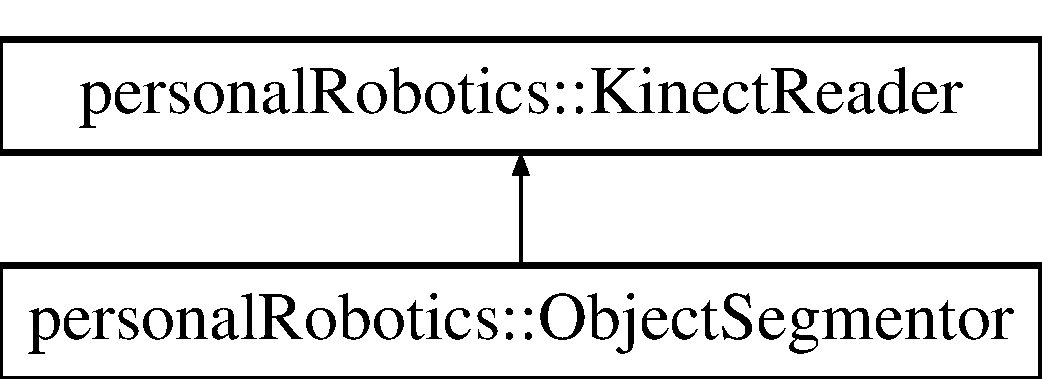
\includegraphics[height=2.000000cm]{d2/d0e/classpersonal_robotics_1_1_kinect_reader}
\end{center}
\end{figure}
\subsection*{Public Member Functions}
\begin{DoxyCompactItemize}
\item 
\hyperlink{classpersonal_robotics_1_1_kinect_reader_a69d11390fa49438a1a902c224b7e3b5c}{Kinect\+Reader} ()
\begin{DoxyCompactList}\small\item\em Default constructor. Acquires required interface as the object is constructed. \end{DoxyCompactList}\item 
\hyperlink{classpersonal_robotics_1_1_kinect_reader_a66a9f845a60a1bed3ccf6c7883a47a9c}{$\sim$\+Kinect\+Reader} ()
\begin{DoxyCompactList}\small\item\em Default destructor. Releases acquired interfaces before destruction. \end{DoxyCompactList}\item 
void \hyperlink{classpersonal_robotics_1_1_kinect_reader_a503882cdd6ad197882c0e8c4eab14664}{map\+Infrared\+To\+Color} (std\+::vector$<$ cv\+::\+Point $>$ \&infrared\+Points, std\+::vector$<$ cv\+::\+Point $>$ \&color\+Points, Color\+Space\+Point $\ast$mapping)
\begin{DoxyCompactList}\small\item\em Converts a set of points from depth/infrared frame to color frame. \end{DoxyCompactList}\item 
void \hyperlink{classpersonal_robotics_1_1_kinect_reader_ab4e331adf22016e45341a0a121b31ad7}{poll\+Frames} (bool save)
\begin{DoxyCompactList}\small\item\em Polls for a new frame and generates a point cloud from the depth map. \end{DoxyCompactList}\item 
\hypertarget{classpersonal_robotics_1_1_kinect_reader_a9263a03547aa8f9d401d3e2ad34f5e4f}{}void \hyperlink{classpersonal_robotics_1_1_kinect_reader_a9263a03547aa8f9d401d3e2ad34f5e4f}{kinect\+Thread\+Routine} ()\label{classpersonal_robotics_1_1_kinect_reader_a9263a03547aa8f9d401d3e2ad34f5e4f}

\begin{DoxyCompactList}\small\item\em Continuously polls for new images by calling \hyperlink{classpersonal_robotics_1_1_kinect_reader_ab4e331adf22016e45341a0a121b31ad7}{poll\+Frames()} in a loop. \end{DoxyCompactList}\item 
\hypertarget{classpersonal_robotics_1_1_kinect_reader_adc75d3fe175de9d6fea8b48ae90de06c}{}void \hyperlink{classpersonal_robotics_1_1_kinect_reader_adc75d3fe175de9d6fea8b48ae90de06c}{start\+Kinect} ()\label{classpersonal_robotics_1_1_kinect_reader_adc75d3fe175de9d6fea8b48ae90de06c}

\begin{DoxyCompactList}\small\item\em Spawns a thread to run \hyperlink{classpersonal_robotics_1_1_kinect_reader_a9263a03547aa8f9d401d3e2ad34f5e4f}{kinect\+Thread\+Routine()} to continuosly poll for frames. \end{DoxyCompactList}\item 
\hypertarget{classpersonal_robotics_1_1_kinect_reader_a40ee858f5274108e8b9ad4a13c14cbd2}{}void \hyperlink{classpersonal_robotics_1_1_kinect_reader_a40ee858f5274108e8b9ad4a13c14cbd2}{stop\+Kinect} ()\label{classpersonal_robotics_1_1_kinect_reader_a40ee858f5274108e8b9ad4a13c14cbd2}

\begin{DoxyCompactList}\small\item\em Stops the kinect\+Reader thread and merges it cleanly with the parent thread. \end{DoxyCompactList}\item 
\hypertarget{classpersonal_robotics_1_1_kinect_reader_a03ac1f0fd33411971f34249be1495edb}{}I\+Coordinate\+Mapper $\ast$ \hyperlink{classpersonal_robotics_1_1_kinect_reader_a03ac1f0fd33411971f34249be1495edb}{get\+Coordinate\+Mapper} ()\label{classpersonal_robotics_1_1_kinect_reader_a03ac1f0fd33411971f34249be1495edb}

\begin{DoxyCompactList}\small\item\em Gets a pointer to the coordinate mapper interface acquired during construction of the object. \end{DoxyCompactList}\item 
\hypertarget{classpersonal_robotics_1_1_kinect_reader_afb46f664c9181b8ceb9abdb46afe0482}{}cv\+::\+Mat $\ast$ \hyperlink{classpersonal_robotics_1_1_kinect_reader_afb46f664c9181b8ceb9abdb46afe0482}{get\+Color\+Image\+Ptr} ()\label{classpersonal_robotics_1_1_kinect_reader_afb46f664c9181b8ceb9abdb46afe0482}

\begin{DoxyCompactList}\small\item\em Gets a pointer to the color image matrix. \end{DoxyCompactList}\item 
\hypertarget{classpersonal_robotics_1_1_kinect_reader_aee0181e76408bc5f9a2771dea5890447}{}cv\+::\+Mat $\ast$ \hyperlink{classpersonal_robotics_1_1_kinect_reader_aee0181e76408bc5f9a2771dea5890447}{get\+I\+Rimage\+Ptr} ()\label{classpersonal_robotics_1_1_kinect_reader_aee0181e76408bc5f9a2771dea5890447}

\begin{DoxyCompactList}\small\item\em Gets a pointer to the infrared image matrix. \end{DoxyCompactList}\item 
\hypertarget{classpersonal_robotics_1_1_kinect_reader_ae794fee5a9061c16d40237481f9ed913}{}cv\+::\+Mat $\ast$ \hyperlink{classpersonal_robotics_1_1_kinect_reader_ae794fee5a9061c16d40237481f9ed913}{get\+Depth\+Image\+Ptr} ()\label{classpersonal_robotics_1_1_kinect_reader_ae794fee5a9061c16d40237481f9ed913}

\begin{DoxyCompactList}\small\item\em Gets a pointer to the depth image matrix. \end{DoxyCompactList}\item 
\hypertarget{classpersonal_robotics_1_1_kinect_reader_a92e2afe02efab759262e4638991c285f}{}Camera\+Space\+Point $\ast$ \hyperlink{classpersonal_robotics_1_1_kinect_reader_a92e2afe02efab759262e4638991c285f}{get\+Point\+Cloud\+Ptr} ()\label{classpersonal_robotics_1_1_kinect_reader_a92e2afe02efab759262e4638991c285f}

\begin{DoxyCompactList}\small\item\em Gets a pointer to the point cloud computed by the coordinate mapper. \end{DoxyCompactList}\item 
\hypertarget{classpersonal_robotics_1_1_kinect_reader_aa3490e36da08c2f89908706a76a6508f}{}size\+\_\+t \hyperlink{classpersonal_robotics_1_1_kinect_reader_aa3490e36da08c2f89908706a76a6508f}{get\+Point\+Cloud\+Size} ()\label{classpersonal_robotics_1_1_kinect_reader_aa3490e36da08c2f89908706a76a6508f}

\begin{DoxyCompactList}\small\item\em Gets the size of the point cloud, i.\+e the number of points. It is equal to the number of pixels in depth image. \end{DoxyCompactList}\end{DoxyCompactItemize}
\subsection*{Public Attributes}
\begin{DoxyCompactItemize}
\item 
\hypertarget{classpersonal_robotics_1_1_kinect_reader_a209d0248b8df3f39214a850dd2bd97bb}{}\hyperlink{classpersonal_robotics_1_1_mutex_type}{Mutex\+Bool} \hyperlink{classpersonal_robotics_1_1_kinect_reader_a209d0248b8df3f39214a850dd2bd97bb}{new\+Frame\+Arrived}\label{classpersonal_robotics_1_1_kinect_reader_a209d0248b8df3f39214a850dd2bd97bb}

\begin{DoxyCompactList}\small\item\em Set to true each time a new frame is acquired. The consumer function is responsible to set it to false once the frame is used. \end{DoxyCompactList}\item 
\hypertarget{classpersonal_robotics_1_1_kinect_reader_a9e443388b4e4bbbc5541f89d40a4c80e}{}\hyperlink{classpersonal_robotics_1_1_mutex_type}{Mutex\+Bool} \hyperlink{classpersonal_robotics_1_1_kinect_reader_a9e443388b4e4bbbc5541f89d40a4c80e}{stop\+Kinect\+Flag}\label{classpersonal_robotics_1_1_kinect_reader_a9e443388b4e4bbbc5541f89d40a4c80e}

\begin{DoxyCompactList}\small\item\em Control varibale for the while loop in \hyperlink{classpersonal_robotics_1_1_kinect_reader_a9263a03547aa8f9d401d3e2ad34f5e4f}{kinect\+Thread\+Routine()}. The loop ends and the \hyperlink{classpersonal_robotics_1_1_kinect_reader_afe24150fcff220507b3d9dcd9d0bee97}{reader\+Thread} exits when this is set to true by \hyperlink{classpersonal_robotics_1_1_kinect_reader_a40ee858f5274108e8b9ad4a13c14cbd2}{stop\+Kinect()} function. \end{DoxyCompactList}\item 
\hypertarget{classpersonal_robotics_1_1_kinect_reader_a88b3822051a0e9bfbcf119c67deda0ec}{}\hyperlink{classpersonal_robotics_1_1_mutex_type}{Mutex\+Bool} \hyperlink{classpersonal_robotics_1_1_kinect_reader_a88b3822051a0e9bfbcf119c67deda0ec}{is\+Color\+Allocated}\label{classpersonal_robotics_1_1_kinect_reader_a88b3822051a0e9bfbcf119c67deda0ec}

\begin{DoxyCompactList}\small\item\em This is set to true once when the first frame arrives and the memory to store color image data is allocated based on the size of the image. \end{DoxyCompactList}\item 
\hypertarget{classpersonal_robotics_1_1_kinect_reader_a2f7a2f527563a51aecc274d845345bfd}{}\hyperlink{classpersonal_robotics_1_1_mutex_type}{Mutex\+Bool} \hyperlink{classpersonal_robotics_1_1_kinect_reader_a2f7a2f527563a51aecc274d845345bfd}{is\+Depth\+Allocated}\label{classpersonal_robotics_1_1_kinect_reader_a2f7a2f527563a51aecc274d845345bfd}

\begin{DoxyCompactList}\small\item\em This is set to true once when the first frame arrives and the memory to store depth image data is allocated based on the size of the image. \end{DoxyCompactList}\item 
\hypertarget{classpersonal_robotics_1_1_kinect_reader_ab9238f5c5b09575d866b10ad0ef8ea9f}{}\hyperlink{classpersonal_robotics_1_1_mutex_type}{Mutex\+Bool} \hyperlink{classpersonal_robotics_1_1_kinect_reader_ab9238f5c5b09575d866b10ad0ef8ea9f}{is\+I\+Rallocated}\label{classpersonal_robotics_1_1_kinect_reader_ab9238f5c5b09575d866b10ad0ef8ea9f}

\begin{DoxyCompactList}\small\item\em This is set to true once when the first frame arrives and the memory to store infrared image data is allocated based on the size of the image. \end{DoxyCompactList}\item 
\hypertarget{classpersonal_robotics_1_1_kinect_reader_af8a4fd4f23c05743cf4f5ff5a9e5eb78}{}std\+::mutex \hyperlink{classpersonal_robotics_1_1_kinect_reader_af8a4fd4f23c05743cf4f5ff5a9e5eb78}{rgb\+Mutex}\label{classpersonal_robotics_1_1_kinect_reader_af8a4fd4f23c05743cf4f5ff5a9e5eb78}

\begin{DoxyCompactList}\small\item\em Mutex to prevent race conditions while accessing \hyperlink{classpersonal_robotics_1_1_kinect_reader_a32b1651f2e04d3d53a0f1bd6b0b490a1}{rgb\+Image}. \end{DoxyCompactList}\item 
\hypertarget{classpersonal_robotics_1_1_kinect_reader_a815a1807b9d1f78962840e490715cfbf}{}std\+::mutex \hyperlink{classpersonal_robotics_1_1_kinect_reader_a815a1807b9d1f78962840e490715cfbf}{rgba\+Mutex}\label{classpersonal_robotics_1_1_kinect_reader_a815a1807b9d1f78962840e490715cfbf}

\begin{DoxyCompactList}\small\item\em Mutex to prevent race conditions while accessing \hyperlink{classpersonal_robotics_1_1_kinect_reader_a57e3ccdf857990fca134a3c01898ceb7}{rgba\+Image}. \end{DoxyCompactList}\item 
\hypertarget{classpersonal_robotics_1_1_kinect_reader_a706d092b43c447084628ae31444006f5}{}std\+::mutex \hyperlink{classpersonal_robotics_1_1_kinect_reader_a706d092b43c447084628ae31444006f5}{depth\+Mutex}\label{classpersonal_robotics_1_1_kinect_reader_a706d092b43c447084628ae31444006f5}

\begin{DoxyCompactList}\small\item\em Mutex to prevent race conditions while accessing \hyperlink{classpersonal_robotics_1_1_kinect_reader_a4bfa3f18889f77253a76ecd2a6999e60}{depth\+Image}. \end{DoxyCompactList}\item 
\hypertarget{classpersonal_robotics_1_1_kinect_reader_adcd2d452bf2355b4142083201c23f024}{}std\+::mutex \hyperlink{classpersonal_robotics_1_1_kinect_reader_adcd2d452bf2355b4142083201c23f024}{ir\+Mutex}\label{classpersonal_robotics_1_1_kinect_reader_adcd2d452bf2355b4142083201c23f024}

\begin{DoxyCompactList}\small\item\em Mutex to prevent race conditions while accessing \hyperlink{classpersonal_robotics_1_1_kinect_reader_af191fde626809b8b09fd062de68df184}{ir\+Image}. \end{DoxyCompactList}\item 
\hypertarget{classpersonal_robotics_1_1_kinect_reader_a37b014e866d224763ea9675c0056a3d3}{}std\+::mutex \hyperlink{classpersonal_robotics_1_1_kinect_reader_a37b014e866d224763ea9675c0056a3d3}{point\+Cloud\+Mutex}\label{classpersonal_robotics_1_1_kinect_reader_a37b014e866d224763ea9675c0056a3d3}

\begin{DoxyCompactList}\small\item\em Mutex to prevent race conditions while accessing \hyperlink{classpersonal_robotics_1_1_kinect_reader_a0340f3ac6506c0205420120ba60f6614}{point\+Cloud\+Ptr}. \end{DoxyCompactList}\item 
\hypertarget{classpersonal_robotics_1_1_kinect_reader_a5c3da75401f463259923330d4dcb51c6}{}std\+::mutex \hyperlink{classpersonal_robotics_1_1_kinect_reader_a5c3da75401f463259923330d4dcb51c6}{depth2color\+Mapping\+Mutex}\label{classpersonal_robotics_1_1_kinect_reader_a5c3da75401f463259923330d4dcb51c6}

\begin{DoxyCompactList}\small\item\em Mutex to prevent race conditions while accessing \hyperlink{classpersonal_robotics_1_1_kinect_reader_a1c33dad149a819407956d19be1fb2966}{depth2color\+Mapping\+Ptr}. \end{DoxyCompactList}\end{DoxyCompactItemize}
\subsection*{Protected Attributes}
\begin{DoxyCompactItemize}
\item 
\hypertarget{classpersonal_robotics_1_1_kinect_reader_a3c69a0735db377ac7b88a99921c10d5f}{}I\+Kinect\+Sensor $\ast$ \hyperlink{classpersonal_robotics_1_1_kinect_reader_a3c69a0735db377ac7b88a99921c10d5f}{kinect\+Ptr}\label{classpersonal_robotics_1_1_kinect_reader_a3c69a0735db377ac7b88a99921c10d5f}

\begin{DoxyCompactList}\small\item\em Holds the pointer to the kinect sensor acquired during construction of object. \end{DoxyCompactList}\item 
\hypertarget{classpersonal_robotics_1_1_kinect_reader_ab4f2a7d08cb1b7d4452e6d8e5d28170e}{}I\+Multi\+Source\+Frame\+Reader $\ast$ \hyperlink{classpersonal_robotics_1_1_kinect_reader_ab4f2a7d08cb1b7d4452e6d8e5d28170e}{reader\+Ptr}\label{classpersonal_robotics_1_1_kinect_reader_ab4f2a7d08cb1b7d4452e6d8e5d28170e}

\begin{DoxyCompactList}\small\item\em Holds the pointer to coordinate mapper obtained from the kinect sensor during construction. \end{DoxyCompactList}\item 
\hypertarget{classpersonal_robotics_1_1_kinect_reader_a9970b3d07116313d5503d48a34beb4c1}{}I\+Coordinate\+Mapper $\ast$ \hyperlink{classpersonal_robotics_1_1_kinect_reader_a9970b3d07116313d5503d48a34beb4c1}{coordinate\+Mapper\+Ptr}\label{classpersonal_robotics_1_1_kinect_reader_a9970b3d07116313d5503d48a34beb4c1}

\begin{DoxyCompactList}\small\item\em Holds the pointer to multi-\/source frame reader obtained from the kinect sensor during construction. \end{DoxyCompactList}\item 
\hypertarget{classpersonal_robotics_1_1_kinect_reader_afe24150fcff220507b3d9dcd9d0bee97}{}std\+::thread \hyperlink{classpersonal_robotics_1_1_kinect_reader_afe24150fcff220507b3d9dcd9d0bee97}{reader\+Thread}\label{classpersonal_robotics_1_1_kinect_reader_afe24150fcff220507b3d9dcd9d0bee97}

\begin{DoxyCompactList}\small\item\em Handle to the thread that run \hyperlink{classpersonal_robotics_1_1_kinect_reader_a9263a03547aa8f9d401d3e2ad34f5e4f}{kinect\+Thread\+Routine()}. \end{DoxyCompactList}\item 
\hypertarget{classpersonal_robotics_1_1_kinect_reader_a95d4de164416824564674b8ee0ec97de}{}int \hyperlink{classpersonal_robotics_1_1_kinect_reader_a95d4de164416824564674b8ee0ec97de}{rgb\+Width}\label{classpersonal_robotics_1_1_kinect_reader_a95d4de164416824564674b8ee0ec97de}

\begin{DoxyCompactList}\small\item\em Width of the color image in pixels. \end{DoxyCompactList}\item 
\hypertarget{classpersonal_robotics_1_1_kinect_reader_aafddc6d28c178ff10260b42e1e36c1a8}{}int \hyperlink{classpersonal_robotics_1_1_kinect_reader_aafddc6d28c178ff10260b42e1e36c1a8}{rgb\+Height}\label{classpersonal_robotics_1_1_kinect_reader_aafddc6d28c178ff10260b42e1e36c1a8}

\begin{DoxyCompactList}\small\item\em Height of the color image in pixels. \end{DoxyCompactList}\item 
\hypertarget{classpersonal_robotics_1_1_kinect_reader_ad18fdd150ee1d257f5ecb2d6bbff34c2}{}int \hyperlink{classpersonal_robotics_1_1_kinect_reader_ad18fdd150ee1d257f5ecb2d6bbff34c2}{depth\+Width}\label{classpersonal_robotics_1_1_kinect_reader_ad18fdd150ee1d257f5ecb2d6bbff34c2}

\begin{DoxyCompactList}\small\item\em Width of the depth image in pixels. \end{DoxyCompactList}\item 
\hypertarget{classpersonal_robotics_1_1_kinect_reader_ab29a8788a51b831ac162367649fe74a8}{}int \hyperlink{classpersonal_robotics_1_1_kinect_reader_ab29a8788a51b831ac162367649fe74a8}{depth\+Height}\label{classpersonal_robotics_1_1_kinect_reader_ab29a8788a51b831ac162367649fe74a8}

\begin{DoxyCompactList}\small\item\em Height of the depth image in pixels. \end{DoxyCompactList}\item 
\hypertarget{classpersonal_robotics_1_1_kinect_reader_a32b1651f2e04d3d53a0f1bd6b0b490a1}{}cv\+::\+Mat \hyperlink{classpersonal_robotics_1_1_kinect_reader_a32b1651f2e04d3d53a0f1bd6b0b490a1}{rgb\+Image}\label{classpersonal_robotics_1_1_kinect_reader_a32b1651f2e04d3d53a0f1bd6b0b490a1}

\begin{DoxyCompactList}\small\item\em Holds 3 channel color image(8 bits per channel) extracted from the 4-\/channel R\+G\+B\+A image. \end{DoxyCompactList}\item 
\hypertarget{classpersonal_robotics_1_1_kinect_reader_a57e3ccdf857990fca134a3c01898ceb7}{}cv\+::\+Mat \hyperlink{classpersonal_robotics_1_1_kinect_reader_a57e3ccdf857990fca134a3c01898ceb7}{rgba\+Image}\label{classpersonal_robotics_1_1_kinect_reader_a57e3ccdf857990fca134a3c01898ceb7}

\begin{DoxyCompactList}\small\item\em Holds 4 channel color image(8 bits per channel) as produced by kinect A\+P\+I with an empty alpha channel. \end{DoxyCompactList}\item 
\hypertarget{classpersonal_robotics_1_1_kinect_reader_a4bfa3f18889f77253a76ecd2a6999e60}{}cv\+::\+Mat \hyperlink{classpersonal_robotics_1_1_kinect_reader_a4bfa3f18889f77253a76ecd2a6999e60}{depth\+Image}\label{classpersonal_robotics_1_1_kinect_reader_a4bfa3f18889f77253a76ecd2a6999e60}

\begin{DoxyCompactList}\small\item\em Holds the single channel 16-\/bit depth image. The birghtness of each pixel is equal to its depth expressed in millimeters. \end{DoxyCompactList}\item 
\hypertarget{classpersonal_robotics_1_1_kinect_reader_af191fde626809b8b09fd062de68df184}{}cv\+::\+Mat \hyperlink{classpersonal_robotics_1_1_kinect_reader_af191fde626809b8b09fd062de68df184}{ir\+Image}\label{classpersonal_robotics_1_1_kinect_reader_af191fde626809b8b09fd062de68df184}

\begin{DoxyCompactList}\small\item\em Holds the single channel 16-\/bit grayscale I\+R images. \end{DoxyCompactList}\item 
\hypertarget{classpersonal_robotics_1_1_kinect_reader_a0811f6812e14b90923377cc165e267d4}{}cv\+::\+Mat \hyperlink{classpersonal_robotics_1_1_kinect_reader_a0811f6812e14b90923377cc165e267d4}{dummy}\label{classpersonal_robotics_1_1_kinect_reader_a0811f6812e14b90923377cc165e267d4}

\begin{DoxyCompactList}\small\item\em Holds a dummy image for any misc. use. \end{DoxyCompactList}\item 
\hypertarget{classpersonal_robotics_1_1_kinect_reader_a0340f3ac6506c0205420120ba60f6614}{}Camera\+Space\+Point $\ast$ \hyperlink{classpersonal_robotics_1_1_kinect_reader_a0340f3ac6506c0205420120ba60f6614}{point\+Cloud\+Ptr}\label{classpersonal_robotics_1_1_kinect_reader_a0340f3ac6506c0205420120ba60f6614}

\begin{DoxyCompactList}\small\item\em Array of points expressed in 3\+D camera space. The unit of distance is meter. The points are generated by coordinate mapper based the \hyperlink{classpersonal_robotics_1_1_kinect_reader_a4bfa3f18889f77253a76ecd2a6999e60}{depth\+Image}. \end{DoxyCompactList}\item 
\hypertarget{classpersonal_robotics_1_1_kinect_reader_a1c33dad149a819407956d19be1fb2966}{}Color\+Space\+Point $\ast$ \hyperlink{classpersonal_robotics_1_1_kinect_reader_a1c33dad149a819407956d19be1fb2966}{depth2color\+Mapping\+Ptr}\label{classpersonal_robotics_1_1_kinect_reader_a1c33dad149a819407956d19be1fb2966}

\begin{DoxyCompactList}\small\item\em Holds a mapping of points in \hyperlink{classpersonal_robotics_1_1_kinect_reader_a4bfa3f18889f77253a76ecd2a6999e60}{depth\+Image} to their correspoing points in \hyperlink{classpersonal_robotics_1_1_kinect_reader_a32b1651f2e04d3d53a0f1bd6b0b490a1}{rgb\+Image}. The mapping is a function of the \hyperlink{classpersonal_robotics_1_1_kinect_reader_a4bfa3f18889f77253a76ecd2a6999e60}{depth\+Image} itself. \end{DoxyCompactList}\end{DoxyCompactItemize}


\subsection{Detailed Description}
This class wraps around the basic Kinect 2.\+0 A\+P\+I provided by Microsoft Kinect S\+D\+K and provides a polling based interface to retrieve image frames. The frames are in sync as they are retrieved using a multi-\/source frame reader. This class runs a thread of its own to poll for frames and sets a \hyperlink{}{Mutex\+Bool} when new frames are acquired.

T\+O\+D\+O\+: \begin{DoxyItemize}
\item {\ttfamily Move} the code for acquisiotion of kinect sensor and other interfaces to Start() function in order to make sure that the object constructor is fail proof. \end{DoxyItemize}


Definition at line 26 of file kinect\+Reader.\+h.



\subsection{Constructor \& Destructor Documentation}
\hypertarget{classpersonal_robotics_1_1_kinect_reader_a69d11390fa49438a1a902c224b7e3b5c}{}\index{personal\+Robotics\+::\+Kinect\+Reader@{personal\+Robotics\+::\+Kinect\+Reader}!Kinect\+Reader@{Kinect\+Reader}}
\index{Kinect\+Reader@{Kinect\+Reader}!personal\+Robotics\+::\+Kinect\+Reader@{personal\+Robotics\+::\+Kinect\+Reader}}
\subsubsection[{Kinect\+Reader}]{\setlength{\rightskip}{0pt plus 5cm}personal\+Robotics\+::\+Kinect\+Reader\+::\+Kinect\+Reader (
\begin{DoxyParamCaption}
{}
\end{DoxyParamCaption}
)}\label{classpersonal_robotics_1_1_kinect_reader_a69d11390fa49438a1a902c224b7e3b5c}
Acquires the default kinect sensor and retrieves the coordinate mapper and multi-\/souce frame reader. 

Definition at line 4 of file kinect\+Reader.\+cpp.

\hypertarget{classpersonal_robotics_1_1_kinect_reader_a66a9f845a60a1bed3ccf6c7883a47a9c}{}\index{personal\+Robotics\+::\+Kinect\+Reader@{personal\+Robotics\+::\+Kinect\+Reader}!````~Kinect\+Reader@{$\sim$\+Kinect\+Reader}}
\index{````~Kinect\+Reader@{$\sim$\+Kinect\+Reader}!personal\+Robotics\+::\+Kinect\+Reader@{personal\+Robotics\+::\+Kinect\+Reader}}
\subsubsection[{$\sim$\+Kinect\+Reader}]{\setlength{\rightskip}{0pt plus 5cm}personal\+Robotics\+::\+Kinect\+Reader\+::$\sim$\+Kinect\+Reader (
\begin{DoxyParamCaption}
{}
\end{DoxyParamCaption}
)}\label{classpersonal_robotics_1_1_kinect_reader_a66a9f845a60a1bed3ccf6c7883a47a9c}
Releases acquired interfaces before destruction of object. However, the destructor does not call the Stop() function. Destruction of the object prior to a call for Stop() will may lead to fatal errors. 

Definition at line 41 of file kinect\+Reader.\+cpp.



\subsection{Member Function Documentation}
\hypertarget{classpersonal_robotics_1_1_kinect_reader_a503882cdd6ad197882c0e8c4eab14664}{}\index{personal\+Robotics\+::\+Kinect\+Reader@{personal\+Robotics\+::\+Kinect\+Reader}!map\+Infrared\+To\+Color@{map\+Infrared\+To\+Color}}
\index{map\+Infrared\+To\+Color@{map\+Infrared\+To\+Color}!personal\+Robotics\+::\+Kinect\+Reader@{personal\+Robotics\+::\+Kinect\+Reader}}
\subsubsection[{map\+Infrared\+To\+Color}]{\setlength{\rightskip}{0pt plus 5cm}void personal\+Robotics\+::\+Kinect\+Reader\+::map\+Infrared\+To\+Color (
\begin{DoxyParamCaption}
\item[{std\+::vector$<$ cv\+::\+Point $>$ \&}]{infrared\+Points, }
\item[{std\+::vector$<$ cv\+::\+Point $>$ \&}]{color\+Points, }
\item[{Color\+Space\+Point $\ast$}]{mapping}
\end{DoxyParamCaption}
)}\label{classpersonal_robotics_1_1_kinect_reader_a503882cdd6ad197882c0e8c4eab14664}
Converts a set of points represented in depth/infrared frame to their corresponding point represented in the color frame. 

Definition at line 56 of file kinect\+Reader.\+cpp.

\hypertarget{classpersonal_robotics_1_1_kinect_reader_ab4e331adf22016e45341a0a121b31ad7}{}\index{personal\+Robotics\+::\+Kinect\+Reader@{personal\+Robotics\+::\+Kinect\+Reader}!poll\+Frames@{poll\+Frames}}
\index{poll\+Frames@{poll\+Frames}!personal\+Robotics\+::\+Kinect\+Reader@{personal\+Robotics\+::\+Kinect\+Reader}}
\subsubsection[{poll\+Frames}]{\setlength{\rightskip}{0pt plus 5cm}void personal\+Robotics\+::\+Kinect\+Reader\+::poll\+Frames (
\begin{DoxyParamCaption}
\item[{bool}]{save}
\end{DoxyParamCaption}
)}\label{classpersonal_robotics_1_1_kinect_reader_ab4e331adf22016e45341a0a121b31ad7}
Polls for a new frame and set \hyperlink{classpersonal_robotics_1_1_kinect_reader_a209d0248b8df3f39214a850dd2bd97bb}{new\+Frame\+Arrived} to true if new image frames are acquired. The function uses \hyperlink{classpersonal_robotics_1_1_kinect_reader_af8a4fd4f23c05743cf4f5ff5a9e5eb78}{rgb\+Mutex}, \hyperlink{classpersonal_robotics_1_1_kinect_reader_a815a1807b9d1f78962840e490715cfbf}{rgba\+Mutex}, \hyperlink{classpersonal_robotics_1_1_kinect_reader_a706d092b43c447084628ae31444006f5}{depth\+Mutex}, \hyperlink{classpersonal_robotics_1_1_kinect_reader_adcd2d452bf2355b4142083201c23f024}{ir\+Mutex}, \hyperlink{classpersonal_robotics_1_1_kinect_reader_a37b014e866d224763ea9675c0056a3d3}{point\+Cloud\+Mutex} and \hyperlink{classpersonal_robotics_1_1_kinect_reader_a5c3da75401f463259923330d4dcb51c6}{depth2color\+Mapping\+Mutex} to prevent race conditions while writinng data to \hyperlink{classpersonal_robotics_1_1_kinect_reader_a32b1651f2e04d3d53a0f1bd6b0b490a1}{rgb\+Image}, \hyperlink{classpersonal_robotics_1_1_kinect_reader_a57e3ccdf857990fca134a3c01898ceb7}{rgba\+Image}, \hyperlink{classpersonal_robotics_1_1_kinect_reader_a4bfa3f18889f77253a76ecd2a6999e60}{depth\+Image}, \hyperlink{classpersonal_robotics_1_1_kinect_reader_af191fde626809b8b09fd062de68df184}{ir\+Image}, \hyperlink{classpersonal_robotics_1_1_kinect_reader_a0340f3ac6506c0205420120ba60f6614}{point\+Cloud\+Ptr} and \hyperlink{classpersonal_robotics_1_1_kinect_reader_a1c33dad149a819407956d19be1fb2966}{depth2color\+Mapping\+Ptr} respectively. 

Definition at line 73 of file kinect\+Reader.\+cpp.



The documentation for this class was generated from the following files\+:\begin{DoxyCompactItemize}
\item 
include/kinect\+Reader.\+h\item 
src/kinect\+Reader.\+cpp\end{DoxyCompactItemize}

\hypertarget{classpersonal_robotics_1_1_mutex_type}{}\section{personal\+Robotics\+:\+:Mutex\+Type$<$ T $>$ Class Template Reference}
\label{classpersonal_robotics_1_1_mutex_type}\index{personal\+Robotics\+::\+Mutex\+Type$<$ T $>$@{personal\+Robotics\+::\+Mutex\+Type$<$ T $>$}}
\subsection*{Public Member Functions}
\begin{DoxyCompactItemize}
\item 
\hypertarget{classpersonal_robotics_1_1_mutex_type_af04fa104e774b42f8f70e053e7f9dc18}{}{\bfseries Mutex\+Type} (T t)\label{classpersonal_robotics_1_1_mutex_type_af04fa104e774b42f8f70e053e7f9dc18}

\item 
\hypertarget{classpersonal_robotics_1_1_mutex_type_a32d87352efdb69e486bfd7ebdf8d5255}{}{\bfseries Mutex\+Type} (const \hyperlink{classpersonal_robotics_1_1_mutex_type}{Mutex\+Type}$<$ T $>$ \&obj)\label{classpersonal_robotics_1_1_mutex_type_a32d87352efdb69e486bfd7ebdf8d5255}

\item 
\hypertarget{classpersonal_robotics_1_1_mutex_type_a3cffd1d15ceb2a3f11e2be4363f3eaa5}{}void {\bfseries lock\+Mutex} ()\label{classpersonal_robotics_1_1_mutex_type_a3cffd1d15ceb2a3f11e2be4363f3eaa5}

\item 
\hypertarget{classpersonal_robotics_1_1_mutex_type_ae67a782ecb9d1edbfe7c06b0624254e9}{}void {\bfseries unlock\+Mutex} ()\label{classpersonal_robotics_1_1_mutex_type_ae67a782ecb9d1edbfe7c06b0624254e9}

\item 
\hypertarget{classpersonal_robotics_1_1_mutex_type_a4760b981b8fedccde8d0c2c2449735f1}{}T {\bfseries get} ()\label{classpersonal_robotics_1_1_mutex_type_a4760b981b8fedccde8d0c2c2449735f1}

\item 
\hypertarget{classpersonal_robotics_1_1_mutex_type_a4908187bb76a498509e9020c74d4afe8}{}T $\ast$ {\bfseries get\+Ptr} ()\label{classpersonal_robotics_1_1_mutex_type_a4908187bb76a498509e9020c74d4afe8}

\item 
\hypertarget{classpersonal_robotics_1_1_mutex_type_a9e51362c2cae90ef893eccfdbb63302f}{}void {\bfseries set} (T t)\label{classpersonal_robotics_1_1_mutex_type_a9e51362c2cae90ef893eccfdbb63302f}

\item 
\hypertarget{classpersonal_robotics_1_1_mutex_type_a92a364c6fa77d00dbed0cf354c9e7cc5}{}\hyperlink{classpersonal_robotics_1_1_mutex_type}{Mutex\+Type}$<$ T $>$ {\bfseries operator=} (const T \&param)\label{classpersonal_robotics_1_1_mutex_type_a92a364c6fa77d00dbed0cf354c9e7cc5}

\item 
\hypertarget{classpersonal_robotics_1_1_mutex_type_a278e5a2c4c6263af9b039dfa8d303cf6}{}\hyperlink{classpersonal_robotics_1_1_mutex_type}{Mutex\+Type}$<$ T $>$ \& {\bfseries operator++} ()\label{classpersonal_robotics_1_1_mutex_type_a278e5a2c4c6263af9b039dfa8d303cf6}

\item 
\hypertarget{classpersonal_robotics_1_1_mutex_type_a639e349d4ea67bab3ed94f941575947b}{}\hyperlink{classpersonal_robotics_1_1_mutex_type}{Mutex\+Type}$<$ T $>$ {\bfseries operator++} (int)\label{classpersonal_robotics_1_1_mutex_type_a639e349d4ea67bab3ed94f941575947b}

\item 
\hypertarget{classpersonal_robotics_1_1_mutex_type_a38733878568858e12647d40f99b8b917}{}\hyperlink{classpersonal_robotics_1_1_mutex_type}{Mutex\+Type}$<$ T $>$ \& {\bfseries operator-\/-\/} ()\label{classpersonal_robotics_1_1_mutex_type_a38733878568858e12647d40f99b8b917}

\item 
\hypertarget{classpersonal_robotics_1_1_mutex_type_a95abe111d6ca61a73f8ae6191aada780}{}\hyperlink{classpersonal_robotics_1_1_mutex_type}{Mutex\+Type}$<$ T $>$ {\bfseries operator-\/-\/} (int)\label{classpersonal_robotics_1_1_mutex_type_a95abe111d6ca61a73f8ae6191aada780}

\end{DoxyCompactItemize}
\subsection*{Protected Attributes}
\begin{DoxyCompactItemize}
\item 
\hypertarget{classpersonal_robotics_1_1_mutex_type_a151eabd8d0e9cb3ce6d9f214a298925f}{}std\+::mutex {\bfseries m\+Mutex}\label{classpersonal_robotics_1_1_mutex_type_a151eabd8d0e9cb3ce6d9f214a298925f}

\item 
\hypertarget{classpersonal_robotics_1_1_mutex_type_aca8750364cc6626b9409664693dc683c}{}T {\bfseries data}\label{classpersonal_robotics_1_1_mutex_type_aca8750364cc6626b9409664693dc683c}

\item 
\hypertarget{classpersonal_robotics_1_1_mutex_type_a96b021c61e62fe3d82a190dc6b5652fd}{}int {\bfseries counter}\label{classpersonal_robotics_1_1_mutex_type_a96b021c61e62fe3d82a190dc6b5652fd}

\end{DoxyCompactItemize}


\subsection{Detailed Description}
\subsubsection*{template$<$typename T$>$class personal\+Robotics\+::\+Mutex\+Type$<$ T $>$}



Definition at line 14 of file utilities.\+h.



The documentation for this class was generated from the following file\+:\begin{DoxyCompactItemize}
\item 
include/utilities.\+h\end{DoxyCompactItemize}

\hypertarget{classpersonal_robotics_1_1_object_segmentor}{}\section{personal\+Robotics\+:\+:Object\+Segmentor Class Reference}
\label{classpersonal_robotics_1_1_object_segmentor}\index{personal\+Robotics\+::\+Object\+Segmentor@{personal\+Robotics\+::\+Object\+Segmentor}}
Inheritance diagram for personal\+Robotics\+:\+:Object\+Segmentor\+:\begin{figure}[H]
\begin{center}
\leavevmode
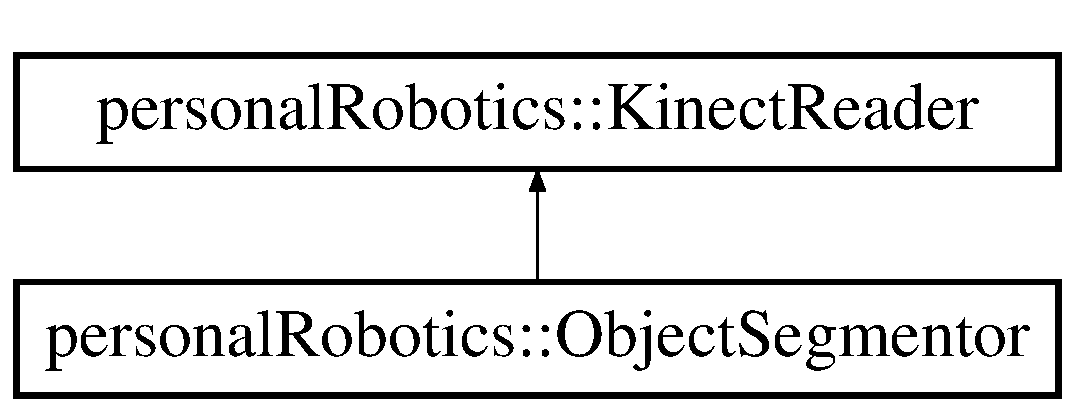
\includegraphics[height=2.000000cm]{d5/d3a/classpersonal_robotics_1_1_object_segmentor}
\end{center}
\end{figure}
\subsection*{Public Member Functions}
\begin{DoxyCompactItemize}
\item 
\hyperlink{classpersonal_robotics_1_1_object_segmentor_a09e8d870efcb51ed0cb0aa95b6c28552}{Object\+Segmentor} ()
\begin{DoxyCompactList}\small\item\em Default constructor. Initializes all the parameters to the defaults specified in \hyperlink{}{setting.\+h} . \end{DoxyCompactList}\item 
\hypertarget{classpersonal_robotics_1_1_object_segmentor_a970e0509a3d2d02ca856e707e3c9d767}{}void \hyperlink{classpersonal_robotics_1_1_object_segmentor_a970e0509a3d2d02ca856e707e3c9d767}{lock\+List} ()\label{classpersonal_robotics_1_1_object_segmentor_a970e0509a3d2d02ca856e707e3c9d767}

\begin{DoxyCompactList}\small\item\em Locks the \hyperlink{classpersonal_robotics_1_1_object_segmentor_aab2136d73a02806e2b09611ed67e65d9}{entity\+List}. The callers should call \hyperlink{classpersonal_robotics_1_1_object_segmentor_a935000c5a4446dc90c768e4fa0c104b9}{unlock\+List()} once the processing is completed. \end{DoxyCompactList}\item 
\hypertarget{classpersonal_robotics_1_1_object_segmentor_a935000c5a4446dc90c768e4fa0c104b9}{}void \hyperlink{classpersonal_robotics_1_1_object_segmentor_a935000c5a4446dc90c768e4fa0c104b9}{unlock\+List} ()\label{classpersonal_robotics_1_1_object_segmentor_a935000c5a4446dc90c768e4fa0c104b9}

\begin{DoxyCompactList}\small\item\em Unlocks the \hyperlink{classpersonal_robotics_1_1_object_segmentor_aab2136d73a02806e2b09611ed67e65d9}{entity\+List}. This method should not be called before a call to \hyperlink{classpersonal_robotics_1_1_object_segmentor_a970e0509a3d2d02ca856e707e3c9d767}{lock\+List()} by the same thread. \end{DoxyCompactList}\item 
\hypertarget{classpersonal_robotics_1_1_object_segmentor_ad5b256a48208fbbb84f8e06b14f5e1c4}{}void \hyperlink{classpersonal_robotics_1_1_object_segmentor_ad5b256a48208fbbb84f8e06b14f5e1c4}{lock\+Pcl} ()\label{classpersonal_robotics_1_1_object_segmentor_ad5b256a48208fbbb84f8e06b14f5e1c4}

\begin{DoxyCompactList}\small\item\em Locks \hyperlink{classpersonal_robotics_1_1_object_segmentor_afd8a8a0d82a7116b78142f4ef3fa3c49}{pcl\+Ptr}. The caller should call \hyperlink{classpersonal_robotics_1_1_object_segmentor_a534a14468aaeb1d3264286b0e070d865}{unlock\+Pcl()} once the processing is completed. \end{DoxyCompactList}\item 
\hypertarget{classpersonal_robotics_1_1_object_segmentor_a534a14468aaeb1d3264286b0e070d865}{}void \hyperlink{classpersonal_robotics_1_1_object_segmentor_a534a14468aaeb1d3264286b0e070d865}{unlock\+Pcl} ()\label{classpersonal_robotics_1_1_object_segmentor_a534a14468aaeb1d3264286b0e070d865}

\begin{DoxyCompactList}\small\item\em Unlocks \hyperlink{classpersonal_robotics_1_1_object_segmentor_afd8a8a0d82a7116b78142f4ef3fa3c49}{pcl\+Ptr}. This method should not be called before a call to \hyperlink{classpersonal_robotics_1_1_object_segmentor_ad5b256a48208fbbb84f8e06b14f5e1c4}{lock\+Pcl()} by the same thread. \end{DoxyCompactList}\item 
\hypertarget{classpersonal_robotics_1_1_object_segmentor_a688bd8c15d467f7ed1c5e25b09524a40}{}std\+::vector$<$ \hyperlink{classpersonal_robotics_1_1_entity}{personal\+Robotics\+::\+Entity} $>$ $\ast$ \hyperlink{classpersonal_robotics_1_1_object_segmentor_a688bd8c15d467f7ed1c5e25b09524a40}{get\+Entity\+List} ()\label{classpersonal_robotics_1_1_object_segmentor_a688bd8c15d467f7ed1c5e25b09524a40}

\begin{DoxyCompactList}\small\item\em Fetches a pointer to \hyperlink{classpersonal_robotics_1_1_object_segmentor_aab2136d73a02806e2b09611ed67e65d9}{entity\+List}. The calling function should also use \hyperlink{classpersonal_robotics_1_1_object_segmentor_a970e0509a3d2d02ca856e707e3c9d767}{lock\+List()} and \hyperlink{classpersonal_robotics_1_1_object_segmentor_a935000c5a4446dc90c768e4fa0c104b9}{unlock\+List()} appropriately to avoid race conditions. \end{DoxyCompactList}\item 
\hypertarget{classpersonal_robotics_1_1_object_segmentor_ac43076bc6a89431f97e847bd38bce43f}{}cv\+::\+Point2f $\ast$ \hyperlink{classpersonal_robotics_1_1_object_segmentor_ac43076bc6a89431f97e847bd38bce43f}{get\+R\+G\+Bpixel\+Size} ()\label{classpersonal_robotics_1_1_object_segmentor_ac43076bc6a89431f97e847bd38bce43f}

\begin{DoxyCompactList}\small\item\em Fetches a pointer to \hyperlink{classpersonal_robotics_1_1_object_segmentor_a7ba1dca4b7433b87ed9028227d0929b3}{rgb\+Pixel\+Size} . \end{DoxyCompactList}\item 
\hypertarget{classpersonal_robotics_1_1_object_segmentor_a60a0e5c08c746773299a400ac8aaec74}{}std\+::vector$<$ \hyperlink{structpersonal_robotics_1_1_i_d_look_up}{I\+D\+Look\+Up} $>$ $\ast$ \hyperlink{classpersonal_robotics_1_1_object_segmentor_a60a0e5c08c746773299a400ac8aaec74}{get\+I\+D\+List} ()\label{classpersonal_robotics_1_1_object_segmentor_a60a0e5c08c746773299a400ac8aaec74}

\begin{DoxyCompactList}\small\item\em Fetches a pointer to \hyperlink{classpersonal_robotics_1_1_object_segmentor_a11e5491339e7f1b543835f10a5daef46}{previous\+I\+D\+List} . \end{DoxyCompactList}\item 
\hypertarget{classpersonal_robotics_1_1_object_segmentor_a412cac1506b709c06548bdfbac1f143d}{}bool \hyperlink{classpersonal_robotics_1_1_object_segmentor_a412cac1506b709c06548bdfbac1f143d}{get\+Static} ()\label{classpersonal_robotics_1_1_object_segmentor_a412cac1506b709c06548bdfbac1f143d}

\begin{DoxyCompactList}\small\item\em Returns true if the scene is static, false otherwise. \end{DoxyCompactList}\item 
void \hyperlink{classpersonal_robotics_1_1_object_segmentor_a44bbf97572b59f392b73fff1fafccc24}{set\+Homography} (cv\+::\+Mat inhomography, int width, int height)
\begin{DoxyCompactList}\small\item\em Sets the homography between the color camera of the kinect and the projected screen followed by, computing the \hyperlink{classpersonal_robotics_1_1_object_segmentor_a2d9b43c69441221cd4b03b61da1ba1ae}{plane\+Normals} . \end{DoxyCompactList}\item 
bool \hyperlink{classpersonal_robotics_1_1_object_segmentor_af4398a1e3f406755ab96787b7d9c50ca}{find\+Table\+Plane} ()
\begin{DoxyCompactList}\small\item\em Estimates the table plane equation using least squares fit with R\+A\+N\+S\+A\+C. \end{DoxyCompactList}\item 
\hypertarget{classpersonal_robotics_1_1_object_segmentor_af02e44cac03022eb39147f63316a2008}{}void \hyperlink{classpersonal_robotics_1_1_object_segmentor_af02e44cac03022eb39147f63316a2008}{start\+Segmentor} ()\label{classpersonal_robotics_1_1_object_segmentor_af02e44cac03022eb39147f63316a2008}

\begin{DoxyCompactList}\small\item\em Starts the segmentor thread that runs \hyperlink{classpersonal_robotics_1_1_object_segmentor_a54dffdc44e4b61ee329c7524f5c04ed1}{segmentor\+Thread\+Routine()}. \end{DoxyCompactList}\item 
\hypertarget{classpersonal_robotics_1_1_object_segmentor_a54dffdc44e4b61ee329c7524f5c04ed1}{}void \hyperlink{classpersonal_robotics_1_1_object_segmentor_a54dffdc44e4b61ee329c7524f5c04ed1}{segmentor\+Thread\+Routine} ()\label{classpersonal_robotics_1_1_object_segmentor_a54dffdc44e4b61ee329c7524f5c04ed1}

\begin{DoxyCompactList}\small\item\em Runs \hyperlink{classpersonal_robotics_1_1_object_segmentor_ad2e4795303539fb1cdd9408730e446cc}{plane\+Segment()} in a loop, handling the pausing and stopping of the segmentor. \end{DoxyCompactList}\item 
\hypertarget{classpersonal_robotics_1_1_object_segmentor_a7704862f53318f456f3efd58d007ea3b}{}void \hyperlink{classpersonal_robotics_1_1_object_segmentor_a7704862f53318f456f3efd58d007ea3b}{stop\+Segmentor} ()\label{classpersonal_robotics_1_1_object_segmentor_a7704862f53318f456f3efd58d007ea3b}

\begin{DoxyCompactList}\small\item\em Stops the segmentor\+Thread\+Routine and mergers the thread cleanly with the parent thread. \end{DoxyCompactList}\item 
\hypertarget{classpersonal_robotics_1_1_object_segmentor_a1e86b4a949c644ab5d9d0079f3e57cad}{}void \hyperlink{classpersonal_robotics_1_1_object_segmentor_a1e86b4a949c644ab5d9d0079f3e57cad}{pause\+Segmentor} ()\label{classpersonal_robotics_1_1_object_segmentor_a1e86b4a949c644ab5d9d0079f3e57cad}

\begin{DoxyCompactList}\small\item\em Pauses the production of the \hyperlink{classpersonal_robotics_1_1_object_segmentor_aab2136d73a02806e2b09611ed67e65d9}{. }\end{DoxyCompactList}\item 
\hypertarget{classpersonal_robotics_1_1_object_segmentor_ab65274e8f1119d39c80e4e0727432336}{}void \hyperlink{classpersonal_robotics_1_1_object_segmentor_ab65274e8f1119d39c80e4e0727432336}{resume\+Segmentor} ()\label{classpersonal_robotics_1_1_object_segmentor_ab65274e8f1119d39c80e4e0727432336}

\begin{DoxyCompactList}\small\item\em Resumes the segmetor. \end{DoxyCompactList}\item 
\hypertarget{classpersonal_robotics_1_1_object_segmentor_ad318d1a55224a9de468b66ffc477ebc6}{}bool \hyperlink{classpersonal_robotics_1_1_object_segmentor_ad318d1a55224a9de468b66ffc477ebc6}{calculate\+Overall\+Change\+In\+Frames} (std\+::vector$<$ \hyperlink{structpersonal_robotics_1_1_i_d_look_up}{I\+D\+Look\+Up} $>$ c\+I\+D\+List)\label{classpersonal_robotics_1_1_object_segmentor_ad318d1a55224a9de468b66ffc477ebc6}

\begin{DoxyCompactList}\small\item\em Returns true if the scene is static for a certain number of frames. \end{DoxyCompactList}\item 
\hypertarget{classpersonal_robotics_1_1_object_segmentor_a742bab296bfdbba8a449163dc7209180}{}float \hyperlink{classpersonal_robotics_1_1_object_segmentor_a742bab296bfdbba8a449163dc7209180}{calculate\+Entity\+Differences} (cv\+::\+Point2f I\+Dcentroid, cv\+::\+Point2f object\+Centroid, float I\+Dangle, float object\+Angle, cv\+::\+Size2f I\+D\+Bounding\+Size, cv\+::\+Size2f object\+Bounding\+Size)\label{classpersonal_robotics_1_1_object_segmentor_a742bab296bfdbba8a449163dc7209180}

\begin{DoxyCompactList}\small\item\em Calculates a score that is a representative of difference between two entities based on pose and size. Smaller the score, better the match. \end{DoxyCompactList}\item 
\hypertarget{classpersonal_robotics_1_1_object_segmentor_a9b69d4969a53e50bcd6c7e59b9ec2b19}{}bool \hyperlink{classpersonal_robotics_1_1_object_segmentor_a9b69d4969a53e50bcd6c7e59b9ec2b19}{on\+Bounding\+Edges} (pcl\+::\+Point\+X\+Y\+Z point)\label{classpersonal_robotics_1_1_object_segmentor_a9b69d4969a53e50bcd6c7e59b9ec2b19}

\begin{DoxyCompactList}\small\item\em Return true if a point is close to the any of the plane in \hyperlink{classpersonal_robotics_1_1_object_segmentor_a2d9b43c69441221cd4b03b61da1ba1ae}{plane\+Normals} . false otherwise. \end{DoxyCompactList}\end{DoxyCompactItemize}
\subsection*{Public Attributes}
\begin{DoxyCompactItemize}
\item 
\hypertarget{classpersonal_robotics_1_1_object_segmentor_a11ae4522730ff37ab707dbacaf9c09fa}{}\hyperlink{classpersonal_robotics_1_1_mutex_type}{Mutex\+Bool} \hyperlink{classpersonal_robotics_1_1_object_segmentor_a11ae4522730ff37ab707dbacaf9c09fa}{new\+List\+Generated}\label{classpersonal_robotics_1_1_object_segmentor_a11ae4522730ff37ab707dbacaf9c09fa}

\begin{DoxyCompactList}\small\item\em Set to true each time the \hyperlink{classpersonal_robotics_1_1_object_segmentor_ad2e4795303539fb1cdd9408730e446cc}{plane\+Segment()} method generates a new list of entities. The consumer function can set it to false after acknowleding the arrival of new list and use it as a signal to wait on. \end{DoxyCompactList}\item 
\hyperlink{classpersonal_robotics_1_1_mutex_type}{Mutex\+Bool} \hyperlink{classpersonal_robotics_1_1_object_segmentor_a28d4c34eee7a10dc1d2bdd9ac5e2835e}{pause\+Thread\+Flag}
\begin{DoxyCompactList}\small\item\em Pauses the segmentor\+Routine() to pause producing new \hyperlink{}{enity\+List} . Refer. \end{DoxyCompactList}\end{DoxyCompactItemize}
\subsection*{Protected Member Functions}
\begin{DoxyCompactItemize}
\item 
void \hyperlink{classpersonal_robotics_1_1_object_segmentor_ad2e4795303539fb1cdd9408730e446cc}{plane\+Segment} ()
\begin{DoxyCompactList}\small\item\em The core routine of the program which segments out objects on the table and generates a list of entities with relavant information. \end{DoxyCompactList}\end{DoxyCompactItemize}
\subsection*{Protected Attributes}
\begin{DoxyCompactItemize}
\item 
\hypertarget{classpersonal_robotics_1_1_object_segmentor_a9289ca41342c0d668e607aedf5e942a9}{}int \hyperlink{classpersonal_robotics_1_1_object_segmentor_a9289ca41342c0d668e607aedf5e942a9}{max\+Ransac\+Iters}\label{classpersonal_robotics_1_1_object_segmentor_a9289ca41342c0d668e607aedf5e942a9}

\begin{DoxyCompactList}\small\item\em Maximum iterations for the R\+A\+N\+S\+A\+C for estimating the table plane. \end{DoxyCompactList}\item 
\hypertarget{classpersonal_robotics_1_1_object_segmentor_ad9c9d0decbab77de45de076291a07c6a}{}float \hyperlink{classpersonal_robotics_1_1_object_segmentor_ad9c9d0decbab77de45de076291a07c6a}{ransac\+Margin}\label{classpersonal_robotics_1_1_object_segmentor_ad9c9d0decbab77de45de076291a07c6a}

\begin{DoxyCompactList}\small\item\em Threshold to distinguish inliers from outliers. Any point is a inlier to a hypothesised plane if the distance between the plane and the point is less than this threshold. \end{DoxyCompactList}\item 
\hypertarget{classpersonal_robotics_1_1_object_segmentor_aebc9c344c5001ab22746b2071783fc2a}{}float \hyperlink{classpersonal_robotics_1_1_object_segmentor_aebc9c344c5001ab22746b2071783fc2a}{dist\+Cutoff}\label{classpersonal_robotics_1_1_object_segmentor_aebc9c344c5001ab22746b2071783fc2a}

\begin{DoxyCompactList}\small\item\em Distance margin within which a point is consider to belong to the table plane. \end{DoxyCompactList}\item 
\hypertarget{classpersonal_robotics_1_1_object_segmentor_aa1f6238eb8f7bc42384f3b2016a13416}{}float \hyperlink{classpersonal_robotics_1_1_object_segmentor_aa1f6238eb8f7bc42384f3b2016a13416}{radial\+Threshold}\label{classpersonal_robotics_1_1_object_segmentor_aa1f6238eb8f7bc42384f3b2016a13416}

\begin{DoxyCompactList}\small\item\em \mbox{[}D\+E\+P\+R\+E\+C\+A\+T\+E\+D\mbox{]} The radius of the circle beyond which the depth pixel are ignored. The distances are computed after accounting for the intrinsics of the depth camera matrix(d = sqrt((X/\+Z)$^\wedge$2 + (Y/\+Z)$^\wedge$2)). \end{DoxyCompactList}\item 
\hypertarget{classpersonal_robotics_1_1_object_segmentor_aff532da1615f30842194f6da1c083423}{}float \hyperlink{classpersonal_robotics_1_1_object_segmentor_aff532da1615f30842194f6da1c083423}{cluster\+Tolerance}\label{classpersonal_robotics_1_1_object_segmentor_aff532da1615f30842194f6da1c083423}

\begin{DoxyCompactList}\small\item\em Threshold for including a point in a cluster. The point is included in the cluster if the distance between the point and its closest point in the cluster is less this threshold. \end{DoxyCompactList}\item 
\hypertarget{classpersonal_robotics_1_1_object_segmentor_aea041b14924056573ba1f3a6f583f9a9}{}int \hyperlink{classpersonal_robotics_1_1_object_segmentor_aea041b14924056573ba1f3a6f583f9a9}{min\+Cluster\+Size}\label{classpersonal_robotics_1_1_object_segmentor_aea041b14924056573ba1f3a6f583f9a9}

\begin{DoxyCompactList}\small\item\em Minimum size of the cluster below which the cluster is drpped. The size of the cluster is the number of points that belong to that cluster. \end{DoxyCompactList}\item 
\hypertarget{classpersonal_robotics_1_1_object_segmentor_a1399221b16239bf902cf1c07536743d3}{}int \hyperlink{classpersonal_robotics_1_1_object_segmentor_a1399221b16239bf902cf1c07536743d3}{max\+Cluster\+Size}\label{classpersonal_robotics_1_1_object_segmentor_a1399221b16239bf902cf1c07536743d3}

\begin{DoxyCompactList}\small\item\em Maazimum size of the cluster beyond which the cluster is dropped for computaional purposes. The size of the cluster is the number of points that belong to that cluster. \end{DoxyCompactList}\item 
\hypertarget{classpersonal_robotics_1_1_object_segmentor_acf97d17ad413314b2fb2c37e23965897}{}float \hyperlink{classpersonal_robotics_1_1_object_segmentor_acf97d17ad413314b2fb2c37e23965897}{min\+Threshold}\label{classpersonal_robotics_1_1_object_segmentor_acf97d17ad413314b2fb2c37e23965897}

\begin{DoxyCompactList}\small\item\em Minimum depth(\+Z) below which the points are rejected. \end{DoxyCompactList}\item 
\hypertarget{classpersonal_robotics_1_1_object_segmentor_a6c231e1c3a430d1df8da3684e9e9e56d}{}float \hyperlink{classpersonal_robotics_1_1_object_segmentor_a6c231e1c3a430d1df8da3684e9e9e56d}{max\+Threshold}\label{classpersonal_robotics_1_1_object_segmentor_a6c231e1c3a430d1df8da3684e9e9e56d}

\begin{DoxyCompactList}\small\item\em Maximum depth(\+Z) beyond which the points are rejected. \end{DoxyCompactList}\item 
\hypertarget{classpersonal_robotics_1_1_object_segmentor_a7c43b8387dd4c3c52fc8a99f6db827e4}{}float \hyperlink{classpersonal_robotics_1_1_object_segmentor_a7c43b8387dd4c3c52fc8a99f6db827e4}{object\+Difference\+Threshold}\label{classpersonal_robotics_1_1_object_segmentor_a7c43b8387dd4c3c52fc8a99f6db827e4}

\begin{DoxyCompactList}\small\item\em Threshold score below which two entities in consecutive frames are considered the same. The score is computed by \hyperlink{classpersonal_robotics_1_1_object_segmentor_a742bab296bfdbba8a449163dc7209180}{calculate\+Entity\+Differences()} function. \end{DoxyCompactList}\item 
\hypertarget{classpersonal_robotics_1_1_object_segmentor_a2cacaff215dc851445d3d111786e2c12}{}float \hyperlink{classpersonal_robotics_1_1_object_segmentor_a2cacaff215dc851445d3d111786e2c12}{object\+Movement\+Threshold}\label{classpersonal_robotics_1_1_object_segmentor_a2cacaff215dc851445d3d111786e2c12}

\begin{DoxyCompactList}\small\item\em Minimum distance the centroid of an entity needs to translate in two cosecutive frames for the entity to be considered non-\/static. \end{DoxyCompactList}\item 
\hypertarget{classpersonal_robotics_1_1_object_segmentor_afd8a8a0d82a7116b78142f4ef3fa3c49}{}pcl\+::\+Point\+Cloud$<$ pcl\+::\+Point\+X\+Y\+Z $>$\+::Ptr \hyperlink{classpersonal_robotics_1_1_object_segmentor_afd8a8a0d82a7116b78142f4ef3fa3c49}{pcl\+Ptr}\label{classpersonal_robotics_1_1_object_segmentor_afd8a8a0d82a7116b78142f4ef3fa3c49}

\begin{DoxyCompactList}\small\item\em Container to store the pruned point cloud. See \hyperlink{classpersonal_robotics_1_1_object_segmentor_a2d9b43c69441221cd4b03b61da1ba1ae}{plane\+Normals}. \end{DoxyCompactList}\item 
\hypertarget{classpersonal_robotics_1_1_object_segmentor_a90ab411e0e2126ae467fe46b3e2a3cf8}{}pcl\+::\+Model\+Coefficients\+::\+Ptr \hyperlink{classpersonal_robotics_1_1_object_segmentor_a90ab411e0e2126ae467fe46b3e2a3cf8}{plane\+Ptr}\label{classpersonal_robotics_1_1_object_segmentor_a90ab411e0e2126ae467fe46b3e2a3cf8}

\begin{DoxyCompactList}\small\item\em Equation of the plane as estimated by \hyperlink{classpersonal_robotics_1_1_object_segmentor_af4398a1e3f406755ab96787b7d9c50ca}{find\+Table\+Plane()} using least squares fit with R\+A\+N\+S\+A\+C for robust estimation. \end{DoxyCompactList}\item 
\hypertarget{classpersonal_robotics_1_1_object_segmentor_aab2136d73a02806e2b09611ed67e65d9}{}std\+::vector$<$ \hyperlink{classpersonal_robotics_1_1_entity}{personal\+Robotics\+::\+Entity} $>$ \hyperlink{classpersonal_robotics_1_1_object_segmentor_aab2136d73a02806e2b09611ed67e65d9}{entity\+List}\label{classpersonal_robotics_1_1_object_segmentor_aab2136d73a02806e2b09611ed67e65d9}

\begin{DoxyCompactList}\small\item\em A list of entities detected in the current scene. \end{DoxyCompactList}\item 
\hypertarget{classpersonal_robotics_1_1_object_segmentor_a1c8c4d3bb2abf7caa077d8f45849f416}{}cv\+::\+Mat \hyperlink{classpersonal_robotics_1_1_object_segmentor_a1c8c4d3bb2abf7caa077d8f45849f416}{homography}\label{classpersonal_robotics_1_1_object_segmentor_a1c8c4d3bb2abf7caa077d8f45849f416}

\begin{DoxyCompactList}\small\item\em The homography set by the function \hyperlink{classpersonal_robotics_1_1_object_segmentor_a44bbf97572b59f392b73fff1fafccc24}{set\+Homography()}. \end{DoxyCompactList}\item 
std\+::vector$<$ cv\+::\+Point3f $>$ \hyperlink{classpersonal_robotics_1_1_object_segmentor_a2d9b43c69441221cd4b03b61da1ba1ae}{plane\+Normals}
\begin{DoxyCompactList}\small\item\em Set of 4 plane normals, expressed in the same coordinate system as the point cloud, that connect the origin of the camera space to the 4 edges of the projected screen. \end{DoxyCompactList}\item 
\hypertarget{classpersonal_robotics_1_1_object_segmentor_a7ba1dca4b7433b87ed9028227d0929b3}{}cv\+::\+Point2f \hyperlink{classpersonal_robotics_1_1_object_segmentor_a7ba1dca4b7433b87ed9028227d0929b3}{rgb\+Pixel\+Size}\label{classpersonal_robotics_1_1_object_segmentor_a7ba1dca4b7433b87ed9028227d0929b3}

\begin{DoxyCompactList}\small\item\em A rough estimate of the rgb pixel size when projected on to the table plane. The size is expressed in mm. \end{DoxyCompactList}\item 
\hypertarget{classpersonal_robotics_1_1_object_segmentor_a11e5491339e7f1b543835f10a5daef46}{}std\+::vector$<$ \hyperlink{structpersonal_robotics_1_1_i_d_look_up}{I\+D\+Look\+Up} $>$ \hyperlink{classpersonal_robotics_1_1_object_segmentor_a11e5491339e7f1b543835f10a5daef46}{previous\+I\+D\+List}\label{classpersonal_robotics_1_1_object_segmentor_a11e5491339e7f1b543835f10a5daef46}

\begin{DoxyCompactList}\small\item\em A list containing characteristic information of the entities in the last frame for the purpose of entity association across frames. \end{DoxyCompactList}\item 
\hypertarget{classpersonal_robotics_1_1_object_segmentor_aee37376bccaeae9e6b36da2faaa9eff0}{}std\+::vector$<$ \hyperlink{structpersonal_robotics_1_1_i_d_look_up}{I\+D\+Look\+Up} $>$ \hyperlink{classpersonal_robotics_1_1_object_segmentor_aee37376bccaeae9e6b36da2faaa9eff0}{current\+I\+D\+List}\label{classpersonal_robotics_1_1_object_segmentor_aee37376bccaeae9e6b36da2faaa9eff0}

\begin{DoxyCompactList}\small\item\em A list containing characteristic information of the entities in the current frame for the purpose of entity association across frames. \end{DoxyCompactList}\item 
\hypertarget{classpersonal_robotics_1_1_object_segmentor_af002f24ebb3f27183bfc0c93aab5cab2}{}std\+::mutex \hyperlink{classpersonal_robotics_1_1_object_segmentor_af002f24ebb3f27183bfc0c93aab5cab2}{pcl\+Ptr\+Lock}\label{classpersonal_robotics_1_1_object_segmentor_af002f24ebb3f27183bfc0c93aab5cab2}

\begin{DoxyCompactList}\small\item\em Mutex to prevent race conditions while accessing \hyperlink{classpersonal_robotics_1_1_object_segmentor_afd8a8a0d82a7116b78142f4ef3fa3c49}{pcl\+Ptr}. \end{DoxyCompactList}\item 
\hypertarget{classpersonal_robotics_1_1_object_segmentor_a05518bed32d4707c6dd608722c1fdd4c}{}std\+::mutex \hyperlink{classpersonal_robotics_1_1_object_segmentor_a05518bed32d4707c6dd608722c1fdd4c}{entity\+List\+Lock}\label{classpersonal_robotics_1_1_object_segmentor_a05518bed32d4707c6dd608722c1fdd4c}

\begin{DoxyCompactList}\small\item\em Mutex to prevent race conditions while accessing \hyperlink{classpersonal_robotics_1_1_object_segmentor_aab2136d73a02806e2b09611ed67e65d9}{entity\+List}. \end{DoxyCompactList}\item 
\hypertarget{classpersonal_robotics_1_1_object_segmentor_a0f9e3d9c51b814f8f6f3f7af9893382e}{}\hyperlink{classpersonal_robotics_1_1_mutex_type}{Mutex\+Bool} \hyperlink{classpersonal_robotics_1_1_object_segmentor_a0f9e3d9c51b814f8f6f3f7af9893382e}{stop\+Segmentor\+Flag}\label{classpersonal_robotics_1_1_object_segmentor_a0f9e3d9c51b814f8f6f3f7af9893382e}

\begin{DoxyCompactList}\small\item\em Control varibale for the while loop in \hyperlink{classpersonal_robotics_1_1_object_segmentor_a54dffdc44e4b61ee329c7524f5c04ed1}{segmentor\+Thread\+Routine()}. The loop ends and the \hyperlink{classpersonal_robotics_1_1_object_segmentor_afa78651f85b2dd6fe132d4c850ab2cef}{segementor\+Thread} exits when this is set to true by \hyperlink{classpersonal_robotics_1_1_object_segmentor_a7704862f53318f456f3efd58d007ea3b}{stop\+Segmentor()} function. \end{DoxyCompactList}\item 
\hypertarget{classpersonal_robotics_1_1_object_segmentor_a9db85709fda1a2926267411e3c9866db}{}\hyperlink{classpersonal_robotics_1_1_mutex_type}{Mutex\+Bool} \hyperlink{classpersonal_robotics_1_1_object_segmentor_a9db85709fda1a2926267411e3c9866db}{homography\+Set\+Flag}\label{classpersonal_robotics_1_1_object_segmentor_a9db85709fda1a2926267411e3c9866db}

\begin{DoxyCompactList}\small\item\em Set to true when homograpgy is set by the \hyperlink{classpersonal_robotics_1_1_object_segmentor_a44bbf97572b59f392b73fff1fafccc24}{set\+Homography()} function. \end{DoxyCompactList}\item 
\hypertarget{classpersonal_robotics_1_1_object_segmentor_afa78651f85b2dd6fe132d4c850ab2cef}{}std\+::thread \hyperlink{classpersonal_robotics_1_1_object_segmentor_afa78651f85b2dd6fe132d4c850ab2cef}{segementor\+Thread}\label{classpersonal_robotics_1_1_object_segmentor_afa78651f85b2dd6fe132d4c850ab2cef}

\begin{DoxyCompactList}\small\item\em Handle to the thread running the \hyperlink{classpersonal_robotics_1_1_object_segmentor_a54dffdc44e4b61ee329c7524f5c04ed1}{segmentor\+Thread\+Routine()}. \end{DoxyCompactList}\item 
\hypertarget{classpersonal_robotics_1_1_object_segmentor_ae2b23b9198ab28786dbac7801aa1d0cb}{}bool \hyperlink{classpersonal_robotics_1_1_object_segmentor_ae2b23b9198ab28786dbac7801aa1d0cb}{frame\+Static}\label{classpersonal_robotics_1_1_object_segmentor_ae2b23b9198ab28786dbac7801aa1d0cb}

\begin{DoxyCompactList}\small\item\em Set to true if all the valid entities in the current frame appear to be static. false otherwise. \end{DoxyCompactList}\item 
\hypertarget{classpersonal_robotics_1_1_object_segmentor_a09017399b3cca7c2715ea406bec511f5}{}bool \hyperlink{classpersonal_robotics_1_1_object_segmentor_a09017399b3cca7c2715ea406bec511f5}{prev\+Frame\+Static}\label{classpersonal_robotics_1_1_object_segmentor_a09017399b3cca7c2715ea406bec511f5}

\begin{DoxyCompactList}\small\item\em Set to true if all the valid entities in the previous frame appeared to be static. false otherwise. \end{DoxyCompactList}\item 
\hypertarget{classpersonal_robotics_1_1_object_segmentor_acdde55937977d3c65574ef6dbc21a47f}{}int \hyperlink{classpersonal_robotics_1_1_object_segmentor_acdde55937977d3c65574ef6dbc21a47f}{object\+Count}\label{classpersonal_robotics_1_1_object_segmentor_acdde55937977d3c65574ef6dbc21a47f}

\begin{DoxyCompactList}\small\item\em Count of valid objects in the frame. \end{DoxyCompactList}\end{DoxyCompactItemize}


\subsection{Detailed Description}


Definition at line 24 of file object\+Segmentation.\+h.



\subsection{Constructor \& Destructor Documentation}
\hypertarget{classpersonal_robotics_1_1_object_segmentor_a09e8d870efcb51ed0cb0aa95b6c28552}{}\index{personal\+Robotics\+::\+Object\+Segmentor@{personal\+Robotics\+::\+Object\+Segmentor}!Object\+Segmentor@{Object\+Segmentor}}
\index{Object\+Segmentor@{Object\+Segmentor}!personal\+Robotics\+::\+Object\+Segmentor@{personal\+Robotics\+::\+Object\+Segmentor}}
\subsubsection[{Object\+Segmentor}]{\setlength{\rightskip}{0pt plus 5cm}personal\+Robotics\+::\+Object\+Segmentor\+::\+Object\+Segmentor (
\begin{DoxyParamCaption}
{}
\end{DoxyParamCaption}
)}\label{classpersonal_robotics_1_1_object_segmentor_a09e8d870efcb51ed0cb0aa95b6c28552}
Constructs the object with the default values as specified in \hyperlink{}{setting.\+h} . Also starts the kinect reader thread by calling \hyperlink{classpersonal_robotics_1_1_kinect_reader_adc75d3fe175de9d6fea8b48ae90de06c}{start\+Kinect()} 

Definition at line 4 of file object\+Segmentation.\+cpp.



\subsection{Member Function Documentation}
\hypertarget{classpersonal_robotics_1_1_object_segmentor_af4398a1e3f406755ab96787b7d9c50ca}{}\index{personal\+Robotics\+::\+Object\+Segmentor@{personal\+Robotics\+::\+Object\+Segmentor}!find\+Table\+Plane@{find\+Table\+Plane}}
\index{find\+Table\+Plane@{find\+Table\+Plane}!personal\+Robotics\+::\+Object\+Segmentor@{personal\+Robotics\+::\+Object\+Segmentor}}
\subsubsection[{find\+Table\+Plane}]{\setlength{\rightskip}{0pt plus 5cm}bool personal\+Robotics\+::\+Object\+Segmentor\+::find\+Table\+Plane (
\begin{DoxyParamCaption}
{}
\end{DoxyParamCaption}
)}\label{classpersonal_robotics_1_1_object_segmentor_af4398a1e3f406755ab96787b7d9c50ca}
Estimates the table plane equation using least squares fit. The outlies are pruned using R\+A\+N\+S\+A\+C. The function assumes that the table top is the most dominant planar feature in the field of view of the kinects depth camera. 

Definition at line 446 of file object\+Segmentation.\+cpp.

\hypertarget{classpersonal_robotics_1_1_object_segmentor_ad2e4795303539fb1cdd9408730e446cc}{}\index{personal\+Robotics\+::\+Object\+Segmentor@{personal\+Robotics\+::\+Object\+Segmentor}!plane\+Segment@{plane\+Segment}}
\index{plane\+Segment@{plane\+Segment}!personal\+Robotics\+::\+Object\+Segmentor@{personal\+Robotics\+::\+Object\+Segmentor}}
\subsubsection[{plane\+Segment}]{\setlength{\rightskip}{0pt plus 5cm}void personal\+Robotics\+::\+Object\+Segmentor\+::plane\+Segment (
\begin{DoxyParamCaption}
{}
\end{DoxyParamCaption}
)\hspace{0.3cm}{\ttfamily [protected]}}\label{classpersonal_robotics_1_1_object_segmentor_ad2e4795303539fb1cdd9408730e446cc}
This is the core routine of the program. The function perfoms the following operations. \begin{DoxyItemize}
\item {\ttfamily Prunes} the point cloud based on the \hyperlink{classpersonal_robotics_1_1_object_segmentor_a2d9b43c69441221cd4b03b61da1ba1ae}{plane\+Normals} to reject all the point outside the region of interest. \item {\ttfamily Perform} plane based segmentation and extract all the points that lie above the table plane. \item {\ttfamily Perform} statistical outlier removal to suppress noise followed by voxel grid based down-\/sampling. \item {\ttfamily Perform} clustering. Each cluster thus formed corresponds to an entity in the scene. \item {\ttfamily Check} the validity of each cluster and rejecting the clusters that are connected to the frustum walls/(\hyperlink{classpersonal_robotics_1_1_object_segmentor_a2d9b43c69441221cd4b03b61da1ba1ae}{plane\+Normals}). \item {\ttfamily Reproject} each cluster onto the R\+G\+B image and compute the centroid, principle axes and 2\+D pose. \item {\ttfamily Match} each cluster\textquotesingle{}s attributes with the attributes of the clusters in the previous frame and create an association between the clusters across the frames. \item {\ttfamily Check} if the scene has come to rest and generate data for each entity in the list of entities. See \hyperlink{}{generate\+Data()}. \end{DoxyItemize}


Definition at line 225 of file object\+Segmentation.\+cpp.

\hypertarget{classpersonal_robotics_1_1_object_segmentor_a44bbf97572b59f392b73fff1fafccc24}{}\index{personal\+Robotics\+::\+Object\+Segmentor@{personal\+Robotics\+::\+Object\+Segmentor}!set\+Homography@{set\+Homography}}
\index{set\+Homography@{set\+Homography}!personal\+Robotics\+::\+Object\+Segmentor@{personal\+Robotics\+::\+Object\+Segmentor}}
\subsubsection[{set\+Homography}]{\setlength{\rightskip}{0pt plus 5cm}void personal\+Robotics\+::\+Object\+Segmentor\+::set\+Homography (
\begin{DoxyParamCaption}
\item[{cv\+::\+Mat}]{inhomography, }
\item[{int}]{width, }
\item[{int}]{height}
\end{DoxyParamCaption}
)}\label{classpersonal_robotics_1_1_object_segmentor_a44bbf97572b59f392b73fff1fafccc24}
Sets the homography between the color camera of the kinect and the projected screen followed by, computing the \hyperlink{classpersonal_robotics_1_1_object_segmentor_a2d9b43c69441221cd4b03b61da1ba1ae}{plane\+Normals} . This routine needs the \hyperlink{classpersonal_robotics_1_1_object_segmentor_a90ab411e0e2126ae467fe46b3e2a3cf8}{plane\+Ptr} be set by \hyperlink{classpersonal_robotics_1_1_object_segmentor_af4398a1e3f406755ab96787b7d9c50ca}{find\+Table\+Plane()} function. 

Definition at line 81 of file object\+Segmentation.\+cpp.



\subsection{Member Data Documentation}
\hypertarget{classpersonal_robotics_1_1_object_segmentor_a28d4c34eee7a10dc1d2bdd9ac5e2835e}{}\index{personal\+Robotics\+::\+Object\+Segmentor@{personal\+Robotics\+::\+Object\+Segmentor}!pause\+Thread\+Flag@{pause\+Thread\+Flag}}
\index{pause\+Thread\+Flag@{pause\+Thread\+Flag}!personal\+Robotics\+::\+Object\+Segmentor@{personal\+Robotics\+::\+Object\+Segmentor}}
\subsubsection[{pause\+Thread\+Flag}]{\setlength{\rightskip}{0pt plus 5cm}{\bf Mutex\+Bool} personal\+Robotics\+::\+Object\+Segmentor\+::pause\+Thread\+Flag}\label{classpersonal_robotics_1_1_object_segmentor_a28d4c34eee7a10dc1d2bdd9ac5e2835e}
\begin{DoxySeeAlso}{See also}
\hyperlink{classpersonal_robotics_1_1_object_segmentor_a1e86b4a949c644ab5d9d0079f3e57cad}{pause\+Segmentor()}, \hyperlink{classpersonal_robotics_1_1_object_segmentor_ab65274e8f1119d39c80e4e0727432336}{resume\+Segmentor()} 
\end{DoxySeeAlso}


Definition at line 106 of file object\+Segmentation.\+h.

\hypertarget{classpersonal_robotics_1_1_object_segmentor_a2d9b43c69441221cd4b03b61da1ba1ae}{}\index{personal\+Robotics\+::\+Object\+Segmentor@{personal\+Robotics\+::\+Object\+Segmentor}!plane\+Normals@{plane\+Normals}}
\index{plane\+Normals@{plane\+Normals}!personal\+Robotics\+::\+Object\+Segmentor@{personal\+Robotics\+::\+Object\+Segmentor}}
\subsubsection[{plane\+Normals}]{\setlength{\rightskip}{0pt plus 5cm}std\+::vector$<$cv\+::\+Point3f$>$ personal\+Robotics\+::\+Object\+Segmentor\+::plane\+Normals\hspace{0.3cm}{\ttfamily [protected]}}\label{classpersonal_robotics_1_1_object_segmentor_a2d9b43c69441221cd4b03b61da1ba1ae}
Set of 4 plane normals, expressed in the same coordinate system as the point cloud, that connect the origin of the camera space to the 4 edges of the projected screen. As the planes pass through the camera center, the d term is 0, giving a complete plane equation. Only points that lie with-\/in the frustum fromed by the four planes are considered for further processing like clustering, etc. by the \hyperlink{classpersonal_robotics_1_1_object_segmentor_ad2e4795303539fb1cdd9408730e446cc}{plane\+Segment()} function. 

Definition at line 53 of file object\+Segmentation.\+h.



The documentation for this class was generated from the following files\+:\begin{DoxyCompactItemize}
\item 
include/object\+Segmentation.\+h\item 
src/object\+Segmentation.\+cpp\end{DoxyCompactItemize}

\hypertarget{structpersonal_robotics_1_1_pose2_dim}{}\section{personal\+Robotics\+:\+:Pose2\+Dim Struct Reference}
\label{structpersonal_robotics_1_1_pose2_dim}\index{personal\+Robotics\+::\+Pose2\+Dim@{personal\+Robotics\+::\+Pose2\+Dim}}
\subsection*{Public Attributes}
\begin{DoxyCompactItemize}
\item 
\hypertarget{structpersonal_robotics_1_1_pose2_dim_aed9dde2eb1c4b6459918862e443d577a}{}cv\+::\+Point2f {\bfseries position}\label{structpersonal_robotics_1_1_pose2_dim_aed9dde2eb1c4b6459918862e443d577a}

\item 
\hypertarget{structpersonal_robotics_1_1_pose2_dim_a7d807be04fa678f9e4204e549512d709}{}float {\bfseries angle}\label{structpersonal_robotics_1_1_pose2_dim_a7d807be04fa678f9e4204e549512d709}

\end{DoxyCompactItemize}


\subsection{Detailed Description}


Definition at line 11 of file entity.\+h.



The documentation for this struct was generated from the following file\+:\begin{DoxyCompactItemize}
\item 
include/entity.\+h\end{DoxyCompactItemize}

\hypertarget{classpersonal_robotics_1_1_socket_exception}{}\section{personal\+Robotics\+:\+:Socket\+Exception Class Reference}
\label{classpersonal_robotics_1_1_socket_exception}\index{personal\+Robotics\+::\+Socket\+Exception@{personal\+Robotics\+::\+Socket\+Exception}}
Inheritance diagram for personal\+Robotics\+:\+:Socket\+Exception\+:\begin{figure}[H]
\begin{center}
\leavevmode
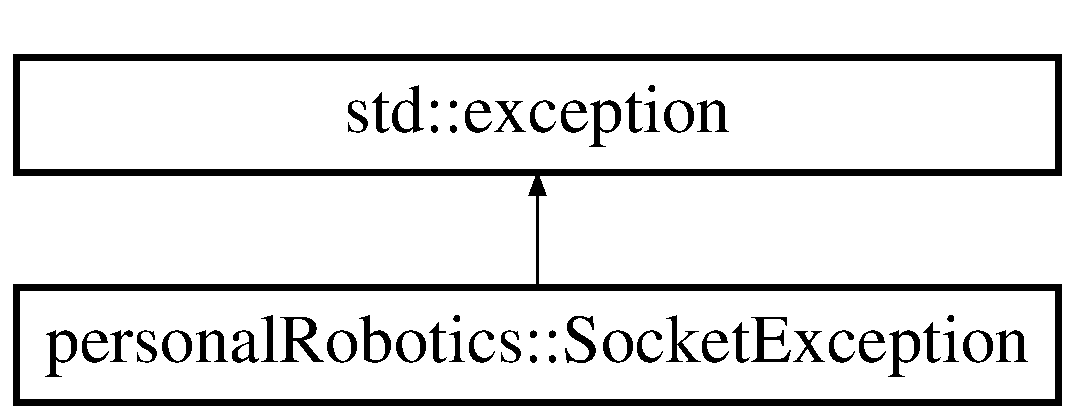
\includegraphics[height=2.000000cm]{dd/d85/classpersonal_robotics_1_1_socket_exception}
\end{center}
\end{figure}
\subsection*{Public Member Functions}
\begin{DoxyCompactItemize}
\item 
\hypertarget{classpersonal_robotics_1_1_socket_exception_a7714cbb4ad1e421a16096a08a3945662}{}{\bfseries Socket\+Exception} (std\+::string s)\label{classpersonal_robotics_1_1_socket_exception_a7714cbb4ad1e421a16096a08a3945662}

\item 
\hypertarget{classpersonal_robotics_1_1_socket_exception_a4f6f8e89b1fe3cad6d498dd193df36e9}{}virtual const char $\ast$ {\bfseries what} () const   throw ()\label{classpersonal_robotics_1_1_socket_exception_a4f6f8e89b1fe3cad6d498dd193df36e9}

\end{DoxyCompactItemize}
\subsection*{Protected Attributes}
\begin{DoxyCompactItemize}
\item 
\hypertarget{classpersonal_robotics_1_1_socket_exception_ac955f7d5829b88ae3f375368dc7dcc01}{}std\+::string {\bfseries ss}\label{classpersonal_robotics_1_1_socket_exception_ac955f7d5829b88ae3f375368dc7dcc01}

\end{DoxyCompactItemize}


\subsection{Detailed Description}


Definition at line 33 of file tcp.\+h.



The documentation for this class was generated from the following file\+:\begin{DoxyCompactItemize}
\item 
include/tcp.\+h\end{DoxyCompactItemize}

\hypertarget{classpersonal_robotics_1_1_tcp}{}\section{personal\+Robotics\+:\+:Tcp Class Reference}
\label{classpersonal_robotics_1_1_tcp}\index{personal\+Robotics\+::\+Tcp@{personal\+Robotics\+::\+Tcp}}
Inheritance diagram for personal\+Robotics\+:\+:Tcp\+:\begin{figure}[H]
\begin{center}
\leavevmode
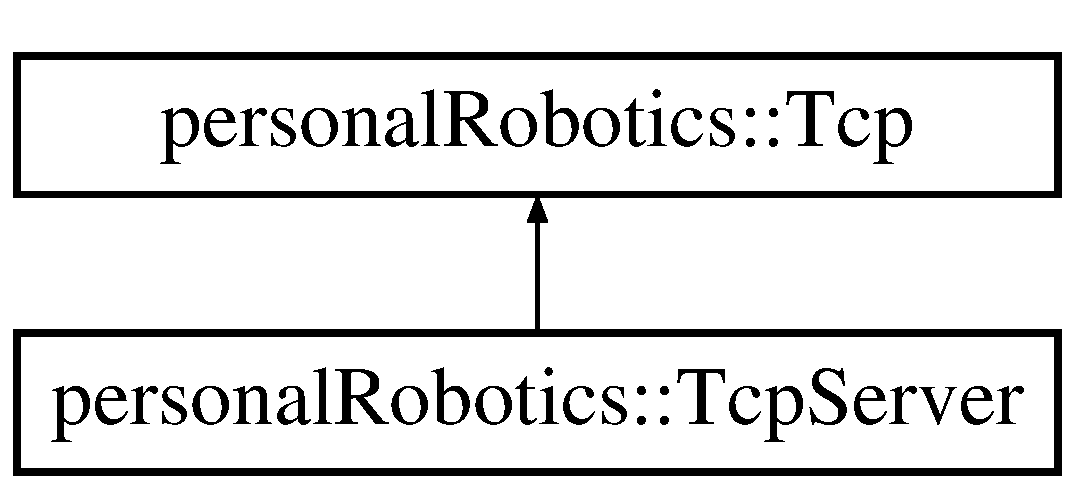
\includegraphics[height=2.000000cm]{de/dd4/classpersonal_robotics_1_1_tcp}
\end{center}
\end{figure}
\subsection*{Public Member Functions}
\begin{DoxyCompactItemize}
\item 
\hypertarget{classpersonal_robotics_1_1_tcp_a44ff0fd6cf8d2374d9c93002c40e2eea}{}void {\bfseries write} (int length, char $\ast$buffer\+Ptr)\label{classpersonal_robotics_1_1_tcp_a44ff0fd6cf8d2374d9c93002c40e2eea}

\item 
\hypertarget{classpersonal_robotics_1_1_tcp_ad66433ec27e099670667dec2b7684543}{}bool {\bfseries read} (int length, char $\ast$buffer\+Ptr)\label{classpersonal_robotics_1_1_tcp_ad66433ec27e099670667dec2b7684543}

\item 
\hypertarget{classpersonal_robotics_1_1_tcp_ad998f98df05e6e9db7bb9f8ab4df9268}{}void {\bfseries async\+Send} (int length, char $\ast$buffer\+Ptr, std\+::mutex \&buffer\+Mutex, bool lock=false, bool unlock=true)\label{classpersonal_robotics_1_1_tcp_ad998f98df05e6e9db7bb9f8ab4df9268}

\item 
\hypertarget{classpersonal_robotics_1_1_tcp_a6442eb84d70478d374685b5638358d57}{}void {\bfseries async\+Read} (int length, char $\ast$buffer\+Ptr, std\+::mutex \&buffer\+Mutex, bool lock=false, bool unlock=true)\label{classpersonal_robotics_1_1_tcp_a6442eb84d70478d374685b5638358d57}

\item 
\hypertarget{classpersonal_robotics_1_1_tcp_acf15c96134bcda539cfef8fe98cba20b}{}void {\bfseries cleanup} ()\label{classpersonal_robotics_1_1_tcp_acf15c96134bcda539cfef8fe98cba20b}

\item 
\hypertarget{classpersonal_robotics_1_1_tcp_a62043b28ed7a7158c10e62e73c552cd7}{}void {\bfseries disconnect} ()\label{classpersonal_robotics_1_1_tcp_a62043b28ed7a7158c10e62e73c552cd7}

\item 
\hypertarget{classpersonal_robotics_1_1_tcp_ade9cef8167d53d198ac84cb1c934d5fd}{}void {\bfseries reset} ()\label{classpersonal_robotics_1_1_tcp_ade9cef8167d53d198ac84cb1c934d5fd}

\end{DoxyCompactItemize}
\subsection*{Public Attributes}
\begin{DoxyCompactItemize}
\item 
\hypertarget{classpersonal_robotics_1_1_tcp_abc65bf1a68082b72e728c018fc1f4a24}{}\hyperlink{classpersonal_robotics_1_1_mutex_type}{Mutex\+Bool} {\bfseries is\+Connected}\label{classpersonal_robotics_1_1_tcp_abc65bf1a68082b72e728c018fc1f4a24}

\item 
\hypertarget{classpersonal_robotics_1_1_tcp_aab864e12f1998209bebd60a0599af30a}{}\hyperlink{classpersonal_robotics_1_1_mutex_type}{Mutex\+Bool} {\bfseries send\+Channel\+Open}\label{classpersonal_robotics_1_1_tcp_aab864e12f1998209bebd60a0599af30a}

\item 
\hypertarget{classpersonal_robotics_1_1_tcp_a2b5c42953b01f452a562e9f83606717e}{}\hyperlink{classpersonal_robotics_1_1_mutex_type}{Mutex\+Bool} {\bfseries recv\+Channel\+Open}\label{classpersonal_robotics_1_1_tcp_a2b5c42953b01f452a562e9f83606717e}

\item 
\hypertarget{classpersonal_robotics_1_1_tcp_a2ac0ad00a81c0f462ffd6d5d87f1a41f}{}\hyperlink{classpersonal_robotics_1_1_mutex_type}{Mutex\+Bool} {\bfseries remote\+Terminated\+Connection}\label{classpersonal_robotics_1_1_tcp_a2ac0ad00a81c0f462ffd6d5d87f1a41f}

\end{DoxyCompactItemize}
\subsection*{Protected Attributes}
\begin{DoxyCompactItemize}
\item 
\hypertarget{classpersonal_robotics_1_1_tcp_a485934a2d97243ae1cf40b0191454975}{}struct addrinfo {\bfseries hints}\label{classpersonal_robotics_1_1_tcp_a485934a2d97243ae1cf40b0191454975}

\item 
\hypertarget{classpersonal_robotics_1_1_tcp_aa22ed1c8a0ba5346baeb6bb99501890b}{}struct addrinfo $\ast$ {\bfseries result}\label{classpersonal_robotics_1_1_tcp_aa22ed1c8a0ba5346baeb6bb99501890b}

\item 
\hypertarget{classpersonal_robotics_1_1_tcp_a3d5f0f540b53d0afeff9351d3c803355}{}struct addrinfo $\ast$ {\bfseries ptr}\label{classpersonal_robotics_1_1_tcp_a3d5f0f540b53d0afeff9351d3c803355}

\item 
\hypertarget{classpersonal_robotics_1_1_tcp_a2da418dc4a1a5f0f5203042faca7d411}{}S\+O\+C\+K\+E\+T {\bfseries data\+Socket}\label{classpersonal_robotics_1_1_tcp_a2da418dc4a1a5f0f5203042faca7d411}

\item 
\hypertarget{classpersonal_robotics_1_1_tcp_acb8526298559a4c1ed190489319ee214}{}std\+::thread {\bfseries send\+Thread}\label{classpersonal_robotics_1_1_tcp_acb8526298559a4c1ed190489319ee214}

\item 
\hypertarget{classpersonal_robotics_1_1_tcp_a60ddfe1ff552e790a686002e1b741d37}{}std\+::thread {\bfseries recv\+Thread}\label{classpersonal_robotics_1_1_tcp_a60ddfe1ff552e790a686002e1b741d37}

\end{DoxyCompactItemize}
\subsection*{Static Protected Attributes}
\begin{DoxyCompactItemize}
\item 
\hypertarget{classpersonal_robotics_1_1_tcp_ab4c9fa15800238ee07083ba03afb9ca3}{}static \hyperlink{classpersonal_robotics_1_1_mutex_type}{Mutex\+Type}$<$ int $>$ {\bfseries socket\+Count} = 0\label{classpersonal_robotics_1_1_tcp_ab4c9fa15800238ee07083ba03afb9ca3}

\end{DoxyCompactItemize}


\subsection{Detailed Description}


Definition at line 51 of file tcp.\+h.



The documentation for this class was generated from the following files\+:\begin{DoxyCompactItemize}
\item 
include/tcp.\+h\item 
src/main.\+cpp\item 
src/tcp.\+cpp\end{DoxyCompactItemize}

\hypertarget{classpersonal_robotics_1_1_tcp_server}{}\section{personal\+Robotics\+:\+:Tcp\+Server Class Reference}
\label{classpersonal_robotics_1_1_tcp_server}\index{personal\+Robotics\+::\+Tcp\+Server@{personal\+Robotics\+::\+Tcp\+Server}}
Inheritance diagram for personal\+Robotics\+:\+:Tcp\+Server\+:\begin{figure}[H]
\begin{center}
\leavevmode
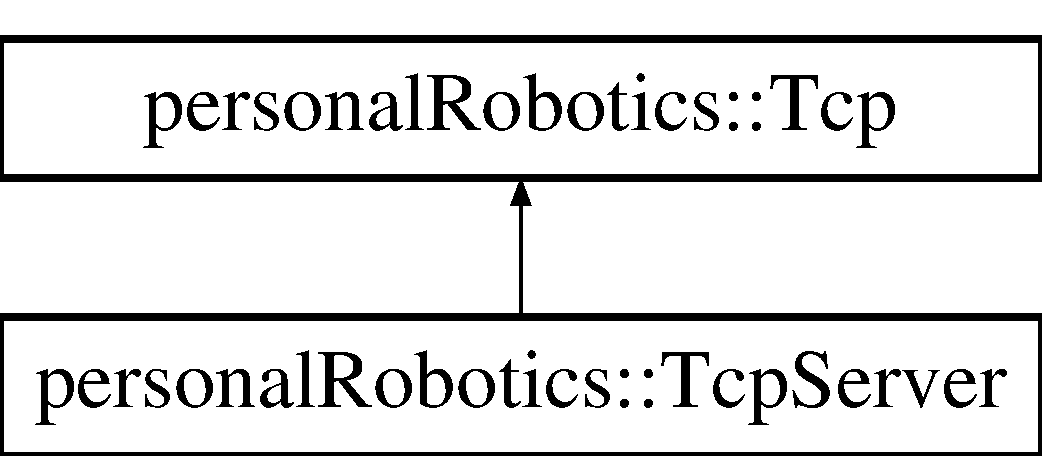
\includegraphics[height=2.000000cm]{d2/d19/classpersonal_robotics_1_1_tcp_server}
\end{center}
\end{figure}
\subsection*{Public Member Functions}
\begin{DoxyCompactItemize}
\item 
\hypertarget{classpersonal_robotics_1_1_tcp_server_a7fc9c4f57dc8768f33a25518a5c08613}{}{\bfseries Tcp\+Server} (int port\+Number, int address\+Family, int socket\+Type=S\+O\+C\+K\+\_\+\+S\+T\+R\+E\+A\+M, int protocol=I\+P\+P\+R\+O\+T\+O\+\_\+\+T\+C\+P, int flags=A\+I\+\_\+\+P\+A\+S\+S\+I\+V\+E)\label{classpersonal_robotics_1_1_tcp_server_a7fc9c4f57dc8768f33a25518a5c08613}

\item 
\hypertarget{classpersonal_robotics_1_1_tcp_server_afebdf28efacfd43b00f22858656b4399}{}{\bfseries Tcp\+Server} (std\+::string port\+Number, int address\+Family, int socket\+Type=S\+O\+C\+K\+\_\+\+S\+T\+R\+E\+A\+M, int protocol=I\+P\+P\+R\+O\+T\+O\+\_\+\+T\+C\+P, int flags=A\+I\+\_\+\+P\+A\+S\+S\+I\+V\+E)\label{classpersonal_robotics_1_1_tcp_server_afebdf28efacfd43b00f22858656b4399}

\item 
\hypertarget{classpersonal_robotics_1_1_tcp_server_aa539f8839511c3d42b96a9e94c6918a1}{}void {\bfseries start} ()\label{classpersonal_robotics_1_1_tcp_server_aa539f8839511c3d42b96a9e94c6918a1}

\item 
\hypertarget{classpersonal_robotics_1_1_tcp_server_a1bd0a6b4cca0339a6727d576027e0767}{}void {\bfseries stop} ()\label{classpersonal_robotics_1_1_tcp_server_a1bd0a6b4cca0339a6727d576027e0767}

\end{DoxyCompactItemize}
\subsection*{Protected Member Functions}
\begin{DoxyCompactItemize}
\item 
\hypertarget{classpersonal_robotics_1_1_tcp_server_a4650c957a6fa66fa4f847aa3b0b82f18}{}void {\bfseries listen\+Routine} ()\label{classpersonal_robotics_1_1_tcp_server_a4650c957a6fa66fa4f847aa3b0b82f18}

\end{DoxyCompactItemize}
\subsection*{Protected Attributes}
\begin{DoxyCompactItemize}
\item 
\hypertarget{classpersonal_robotics_1_1_tcp_server_aae4ed861a52d8e3f9b934f2c78434476}{}S\+O\+C\+K\+E\+T {\bfseries listener}\label{classpersonal_robotics_1_1_tcp_server_aae4ed861a52d8e3f9b934f2c78434476}

\item 
\hypertarget{classpersonal_robotics_1_1_tcp_server_a8363a7709a70654a1317f4ab8f927178}{}\hyperlink{classpersonal_robotics_1_1_mutex_type}{Mutex\+Bool} {\bfseries listener\+Stopped}\label{classpersonal_robotics_1_1_tcp_server_a8363a7709a70654a1317f4ab8f927178}

\item 
\hypertarget{classpersonal_robotics_1_1_tcp_server_a59485a6ad32f739a3ecac1dd7bde0542}{}std\+::thread {\bfseries listener\+Thread}\label{classpersonal_robotics_1_1_tcp_server_a59485a6ad32f739a3ecac1dd7bde0542}

\end{DoxyCompactItemize}
\subsection*{Additional Inherited Members}


\subsection{Detailed Description}


Definition at line 78 of file tcp.\+h.



The documentation for this class was generated from the following files\+:\begin{DoxyCompactItemize}
\item 
include/tcp.\+h\item 
src/tcp.\+cpp\end{DoxyCompactItemize}

\hypertarget{classpersonal_robotics_1_1_timer}{}\section{personal\+Robotics\+:\+:Timer Class Reference}
\label{classpersonal_robotics_1_1_timer}\index{personal\+Robotics\+::\+Timer@{personal\+Robotics\+::\+Timer}}
\subsection*{Public Member Functions}
\begin{DoxyCompactItemize}
\item 
\hypertarget{classpersonal_robotics_1_1_timer_ad1bac9f68d62abd7cdc8c8f2437fc023}{}{\bfseries Timer} (std\+::string tag)\label{classpersonal_robotics_1_1_timer_ad1bac9f68d62abd7cdc8c8f2437fc023}

\item 
\hypertarget{classpersonal_robotics_1_1_timer_a2ac3afcf55bb445e7c9bbec7295cfe0f}{}void {\bfseries tic} ()\label{classpersonal_robotics_1_1_timer_a2ac3afcf55bb445e7c9bbec7295cfe0f}

\item 
\hypertarget{classpersonal_robotics_1_1_timer_a6b86ba949e6f58daba4045390af4e8e7}{}void {\bfseries toc} ()\label{classpersonal_robotics_1_1_timer_a6b86ba949e6f58daba4045390af4e8e7}

\item 
\hypertarget{classpersonal_robotics_1_1_timer_ab3829c97476e592d6a006e671557de4d}{}double {\bfseries get\+Elapsed\+Time} (bool silence)\label{classpersonal_robotics_1_1_timer_ab3829c97476e592d6a006e671557de4d}

\end{DoxyCompactItemize}
\subsection*{Private Attributes}
\begin{DoxyCompactItemize}
\item 
\hypertarget{classpersonal_robotics_1_1_timer_a5329fe5efbe488c87561e207140c51dd}{}clock\+\_\+t {\bfseries m\+Clock}\label{classpersonal_robotics_1_1_timer_a5329fe5efbe488c87561e207140c51dd}

\item 
\hypertarget{classpersonal_robotics_1_1_timer_a43dc8d300ba5e5193f7a5c8babc0f944}{}clock\+\_\+t {\bfseries m\+Start}\label{classpersonal_robotics_1_1_timer_a43dc8d300ba5e5193f7a5c8babc0f944}

\item 
\hypertarget{classpersonal_robotics_1_1_timer_af61b6d78dba3462912218f0a26aef2ab}{}clock\+\_\+t {\bfseries m\+End}\label{classpersonal_robotics_1_1_timer_af61b6d78dba3462912218f0a26aef2ab}

\item 
\hypertarget{classpersonal_robotics_1_1_timer_a25b18e8f5cec8ed7a91038e3d629a805}{}std\+::string {\bfseries m\+Tag}\label{classpersonal_robotics_1_1_timer_a25b18e8f5cec8ed7a91038e3d629a805}

\end{DoxyCompactItemize}


\subsection{Detailed Description}


Definition at line 10 of file timer.\+h.



The documentation for this class was generated from the following files\+:\begin{DoxyCompactItemize}
\item 
include/timer.\+h\item 
src/timer.\+cpp\end{DoxyCompactItemize}

%--- End generated contents ---

% Index
\backmatter
\newpage
\phantomsection
\clearemptydoublepage
\addcontentsline{toc}{chapter}{Index}
\printindex

\end{document}
